\documentclass[12pt, a4paper, oneside]{book}

% Language setting
\usepackage[english]{babel}
\usepackage{setspace}
% Set page size and margins
% Replace `letterpaper' with `a4paper' for UK/EU standard size
\usepackage[a4paper,top=2cm,bottom=2cm,left=3cm,right=3cm,marginparwidth=1.75cm]{geometry}

% Useful packages
\usepackage{amsmath}
\usepackage{graphicx}
\usepackage[colorlinks=true, allcolors=blue]{hyperref}

\usepackage{csquotes}

\usepackage{float}
\usepackage{fix-cm}
\usepackage[table]{xcolor}
\usepackage{titlesec}
\usepackage{soul, color}
\definecolor{gray75}{gray}{0.75}
\newcommand{\hsp}{\hspace{0pt}}
\titleformat{\chapter}[hang]{\flushright
\fontseries{b}\fontsize{80}{100}\selectfont}{\fontseries{b}\fontsize{100}{130}\selectfont \textcolor{gray75}\thechapter\hsp}{0pt}{\Huge\bfseries}[]

\usepackage{tabularx}

\title{DevOps, Software Evolution and Software Maintenance, BSc (Spring 2024)}
\author{Course code: BSDSESM1KU}




\begin{document}

\begin{minipage}{\textwidth}
\maketitle

\begin{center}
    Exam Assignment by: \\
    \hfill \break
    \bgroup
    \def\arraystretch{1.5}%
    \begin{tabularx}{0.8\textwidth} { 
      | >{\centering\arraybackslash}X 
      | >{\centering\arraybackslash}X | }
     \hline
     \cellcolor[HTML]{EFEFEF} Student & \cellcolor[HTML]{EFEFEF} Email \\
     \hline
     Daria Damian & dard@itu.dk \\
     \hline
     Hallgrímur Jónas Jensson & hajj@itu.dk \\
    \hline
     Mathias E. L. Rasmussen & memr@itu.dk \\
    \hline
     Max-Emil Smith Thorius & maxt@itu.dk \\
    \hline
    Fujie Mei & fume@itu.dk \\
    \hline
    \end{tabularx}
    \egroup
\end{center}
\end{minipage}

\tableofcontents

\chapter{System's Perspective}
\label{chap:System's Perspective}

\section{Design and architecture of the Minitwit system}
\label{sec:Design and architecture of the Minitwit system}


% ITU-MiniTwit is designed as a microservices' architecture, leveraging containerization to ensure isolation, ease of deployment, and scalability. The system's architecture facilitates independent development and service deployment, enhancing maintenance and testing capabilities.
% \begin{figure}[h]
%     \centering
%     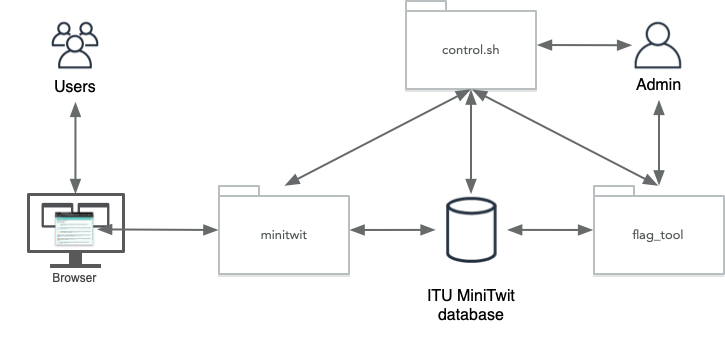
\includegraphics[width=\textwidth]{images/ITU-minitwit-architecture.png}
%     \caption{High-level ITU-MiniTwit architecture}
% \end{figure}\\

The following includes three abstractions of the system to understand the overall architecture better: the relations between the different servers, the relations between the different containers on the \textit{webserver} hosting the main application, and the relations between the different packages in the main web application.

\subsection{Servers}
The system includes four servers that serve different purposes, depicted in Figure \ref{fig:uml-servers}.
The \textit{webserver} is where the main application and the API reside. and the \textit{dbserver} hosts the Postgres database.
This connection is established with GORM, an ORM package for Golang that facilitates the connection from the app and API.
Finally, the two worker servers are backup replicas of the \textit{webserver} to help ensure its availability, connected to the \textit{webserver} in a Docker Swarm environment with the 2 overlay networks: \textit{ingress}, which ensures load balancing, and \textit{minitwit-network}, which allows communication among the Docker daemons.

\begin{figure}[H]
    \centering
    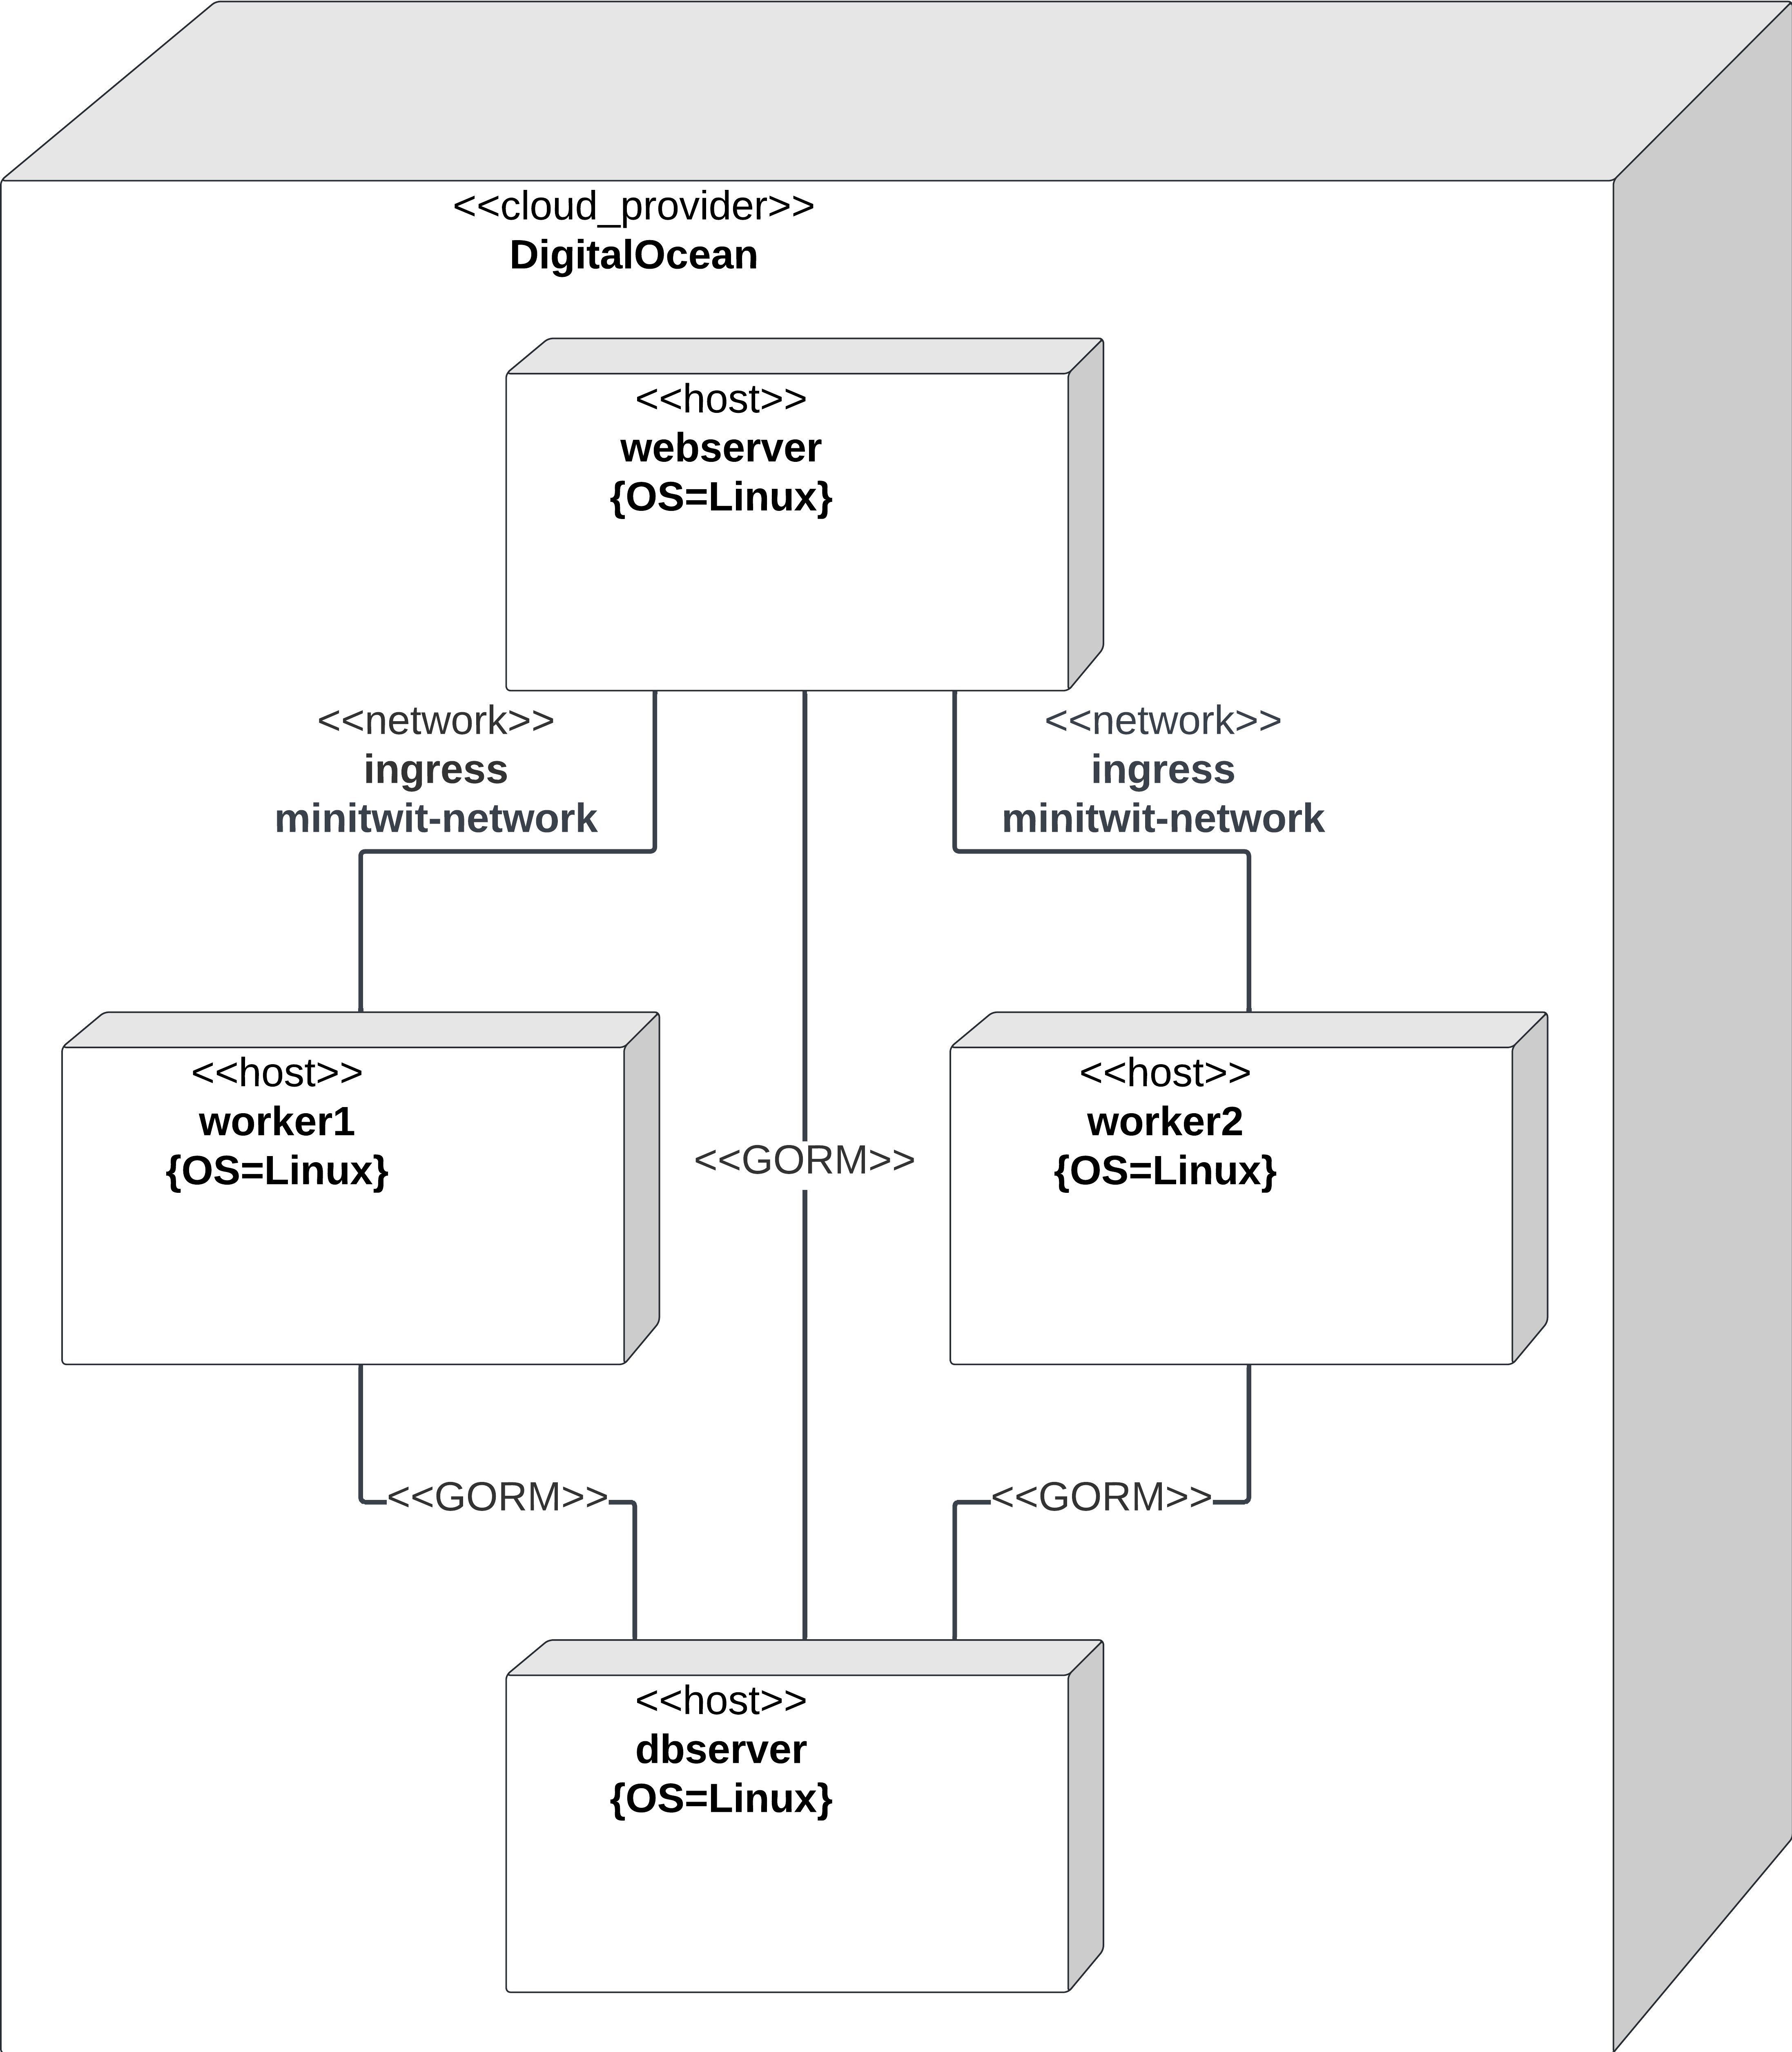
\includegraphics[width=0.6\linewidth]{images/uml-component-servers.png}
    \caption{Diagram displaying the different servers in the architecture and their relations.}
    \label{fig:uml-servers}
\end{figure}

\subsection{Containers}
Zooming in on the \textit{webserver} reveals 2 different networks and 9 different containers running on this server.
Figure \ref{fig:uml-containers} displays the containers running on the server.

\begin{figure}[H]
    \centering
    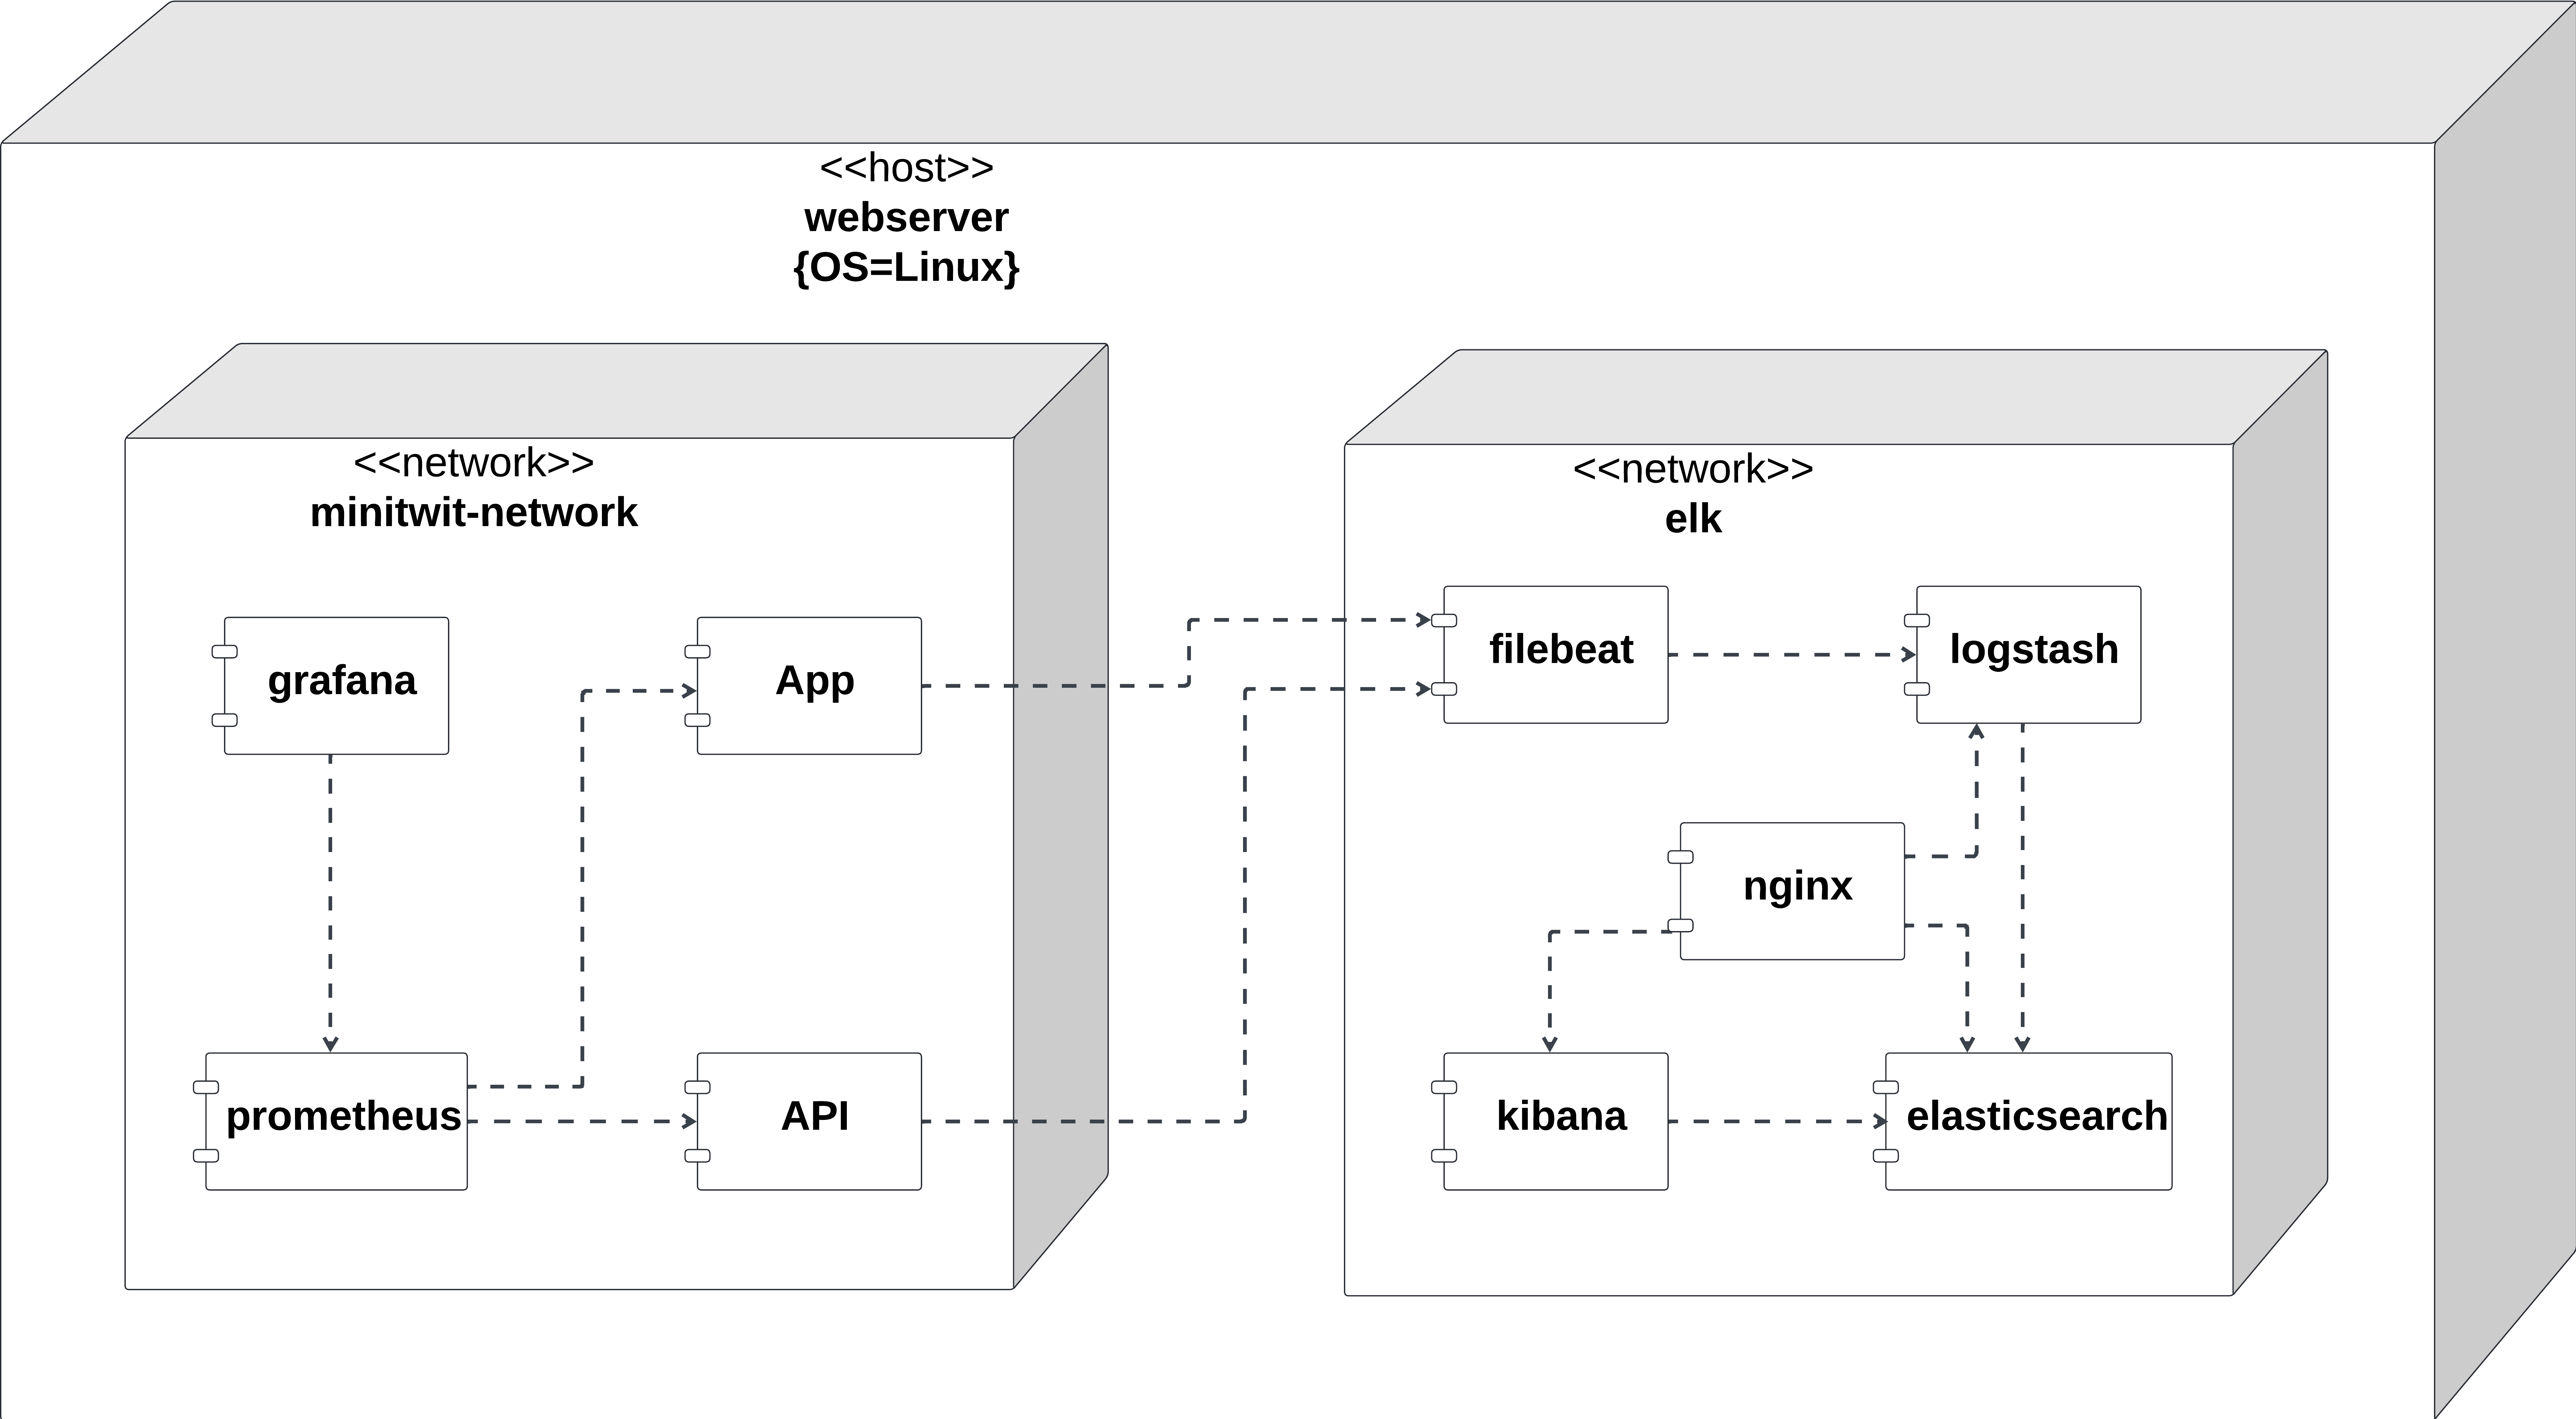
\includegraphics[width=0.8\linewidth]{images/uml-component-containers.png}
    \caption{Component diagram emphasizing the different containers in the architecture and their relations}
    \label{fig:uml-containers}
\end{figure}

\subsection{App}
The following describes the structure of the \textit{App} container displayed in the services.
It includes several packages, all located in the src directory.
A package diagram that visualizes the app's structure is displayed in Figure \ref{fig:package-diagram-app}.
\textit{main.go} is the executed file, which sets up the templates in the \textit{Web} package, establishes database connection with the \textit{Database} package, and sets up controllers in the \textit{Controller} package to endpoints.
The \textit{Controller} package queries the database with the \textit{Database} package, adds popup notifications with the \textit{Flash} package, and creates ORM models with the\textit{Models} package.

\begin{figure}[H]
    \centering
    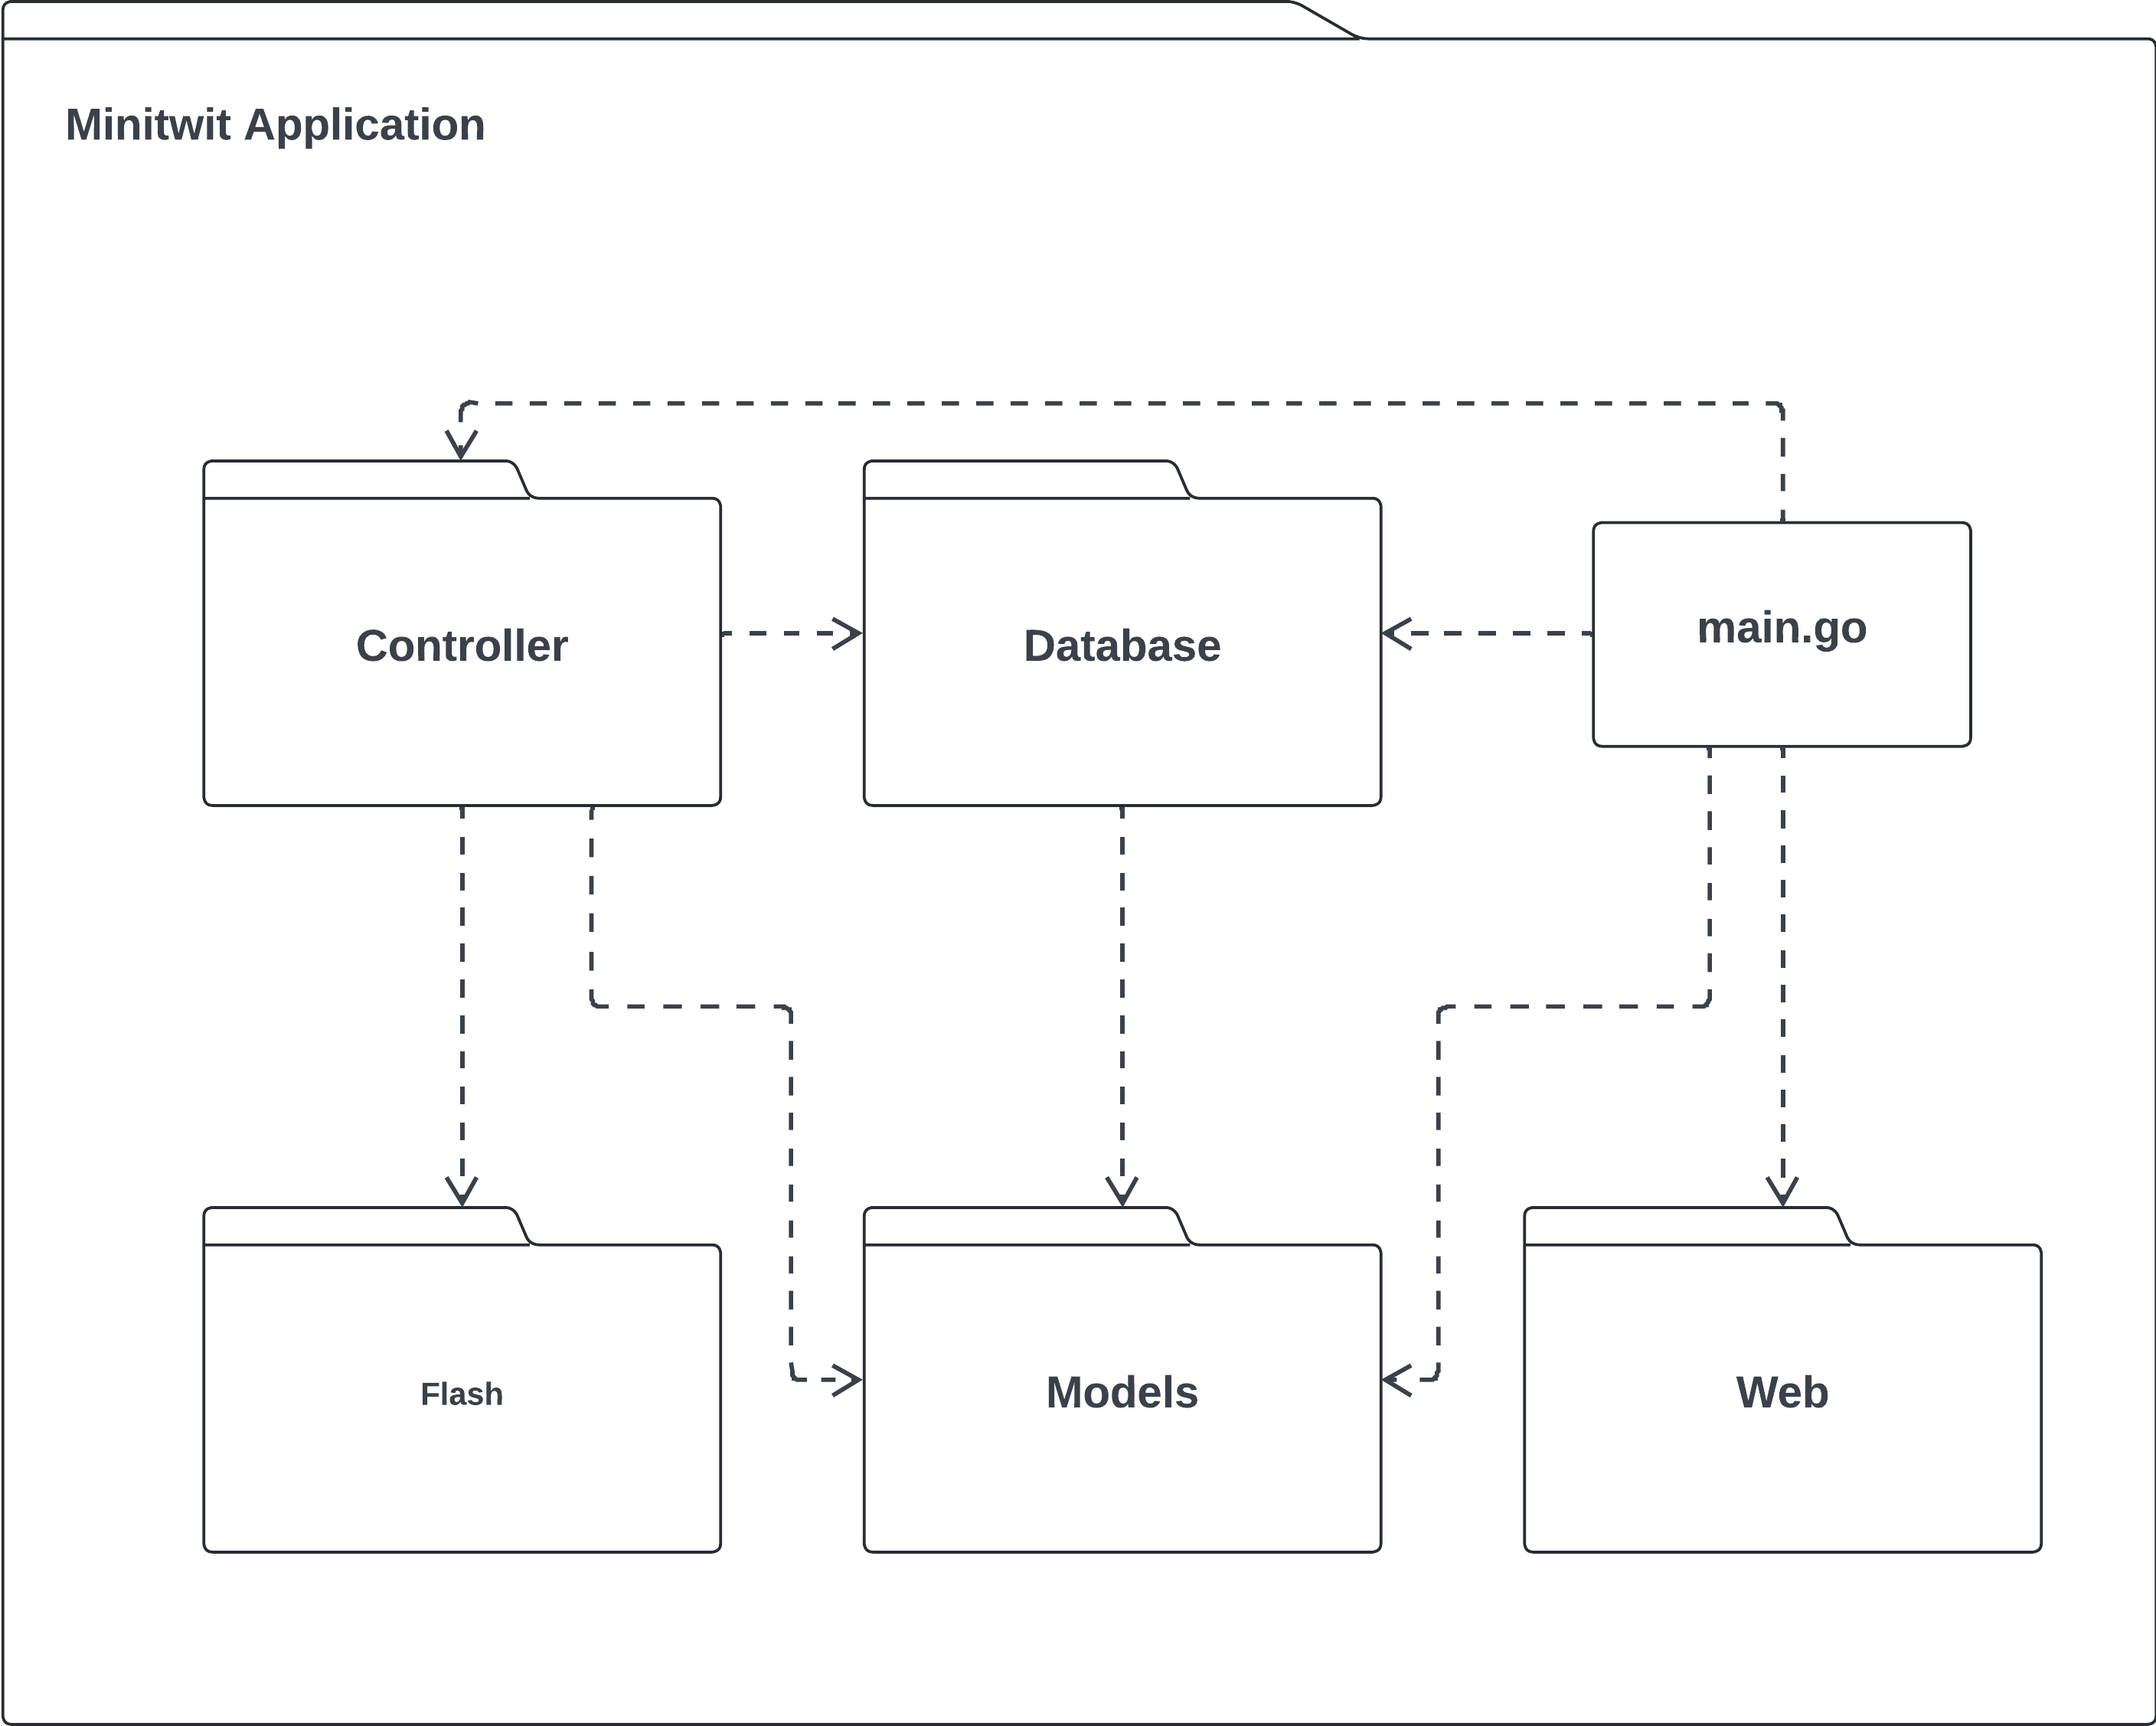
\includegraphics[width=0.6\linewidth]{images/uml-package-app.png}
    \caption{Package diagram of the main application running on the App service}
    \label{fig:package-diagram-app}
\end{figure}

\section{Dependencies of the Minitwit system}

This section will detail all the technologies, tools, and external services our system depends on, structured into categories for clarity.

\subsection{Monitoring}\label{sec:monitoring-architecture}
The system is monitored with Grafana and Prometheus tools, with the stack depicted in Figure \ref{fig:monitoring-stack}.
Prometheus is the data collector, pulling metrics from the app and API.
Grafana queries these metrics and visualizes relevant stats for maintenance.
Furthermore, Grafana also connects to the database to retrieve basic information about the tables in the database.

\begin{figure}[H]
    \centering
    \hbox{\hspace{-5em}
    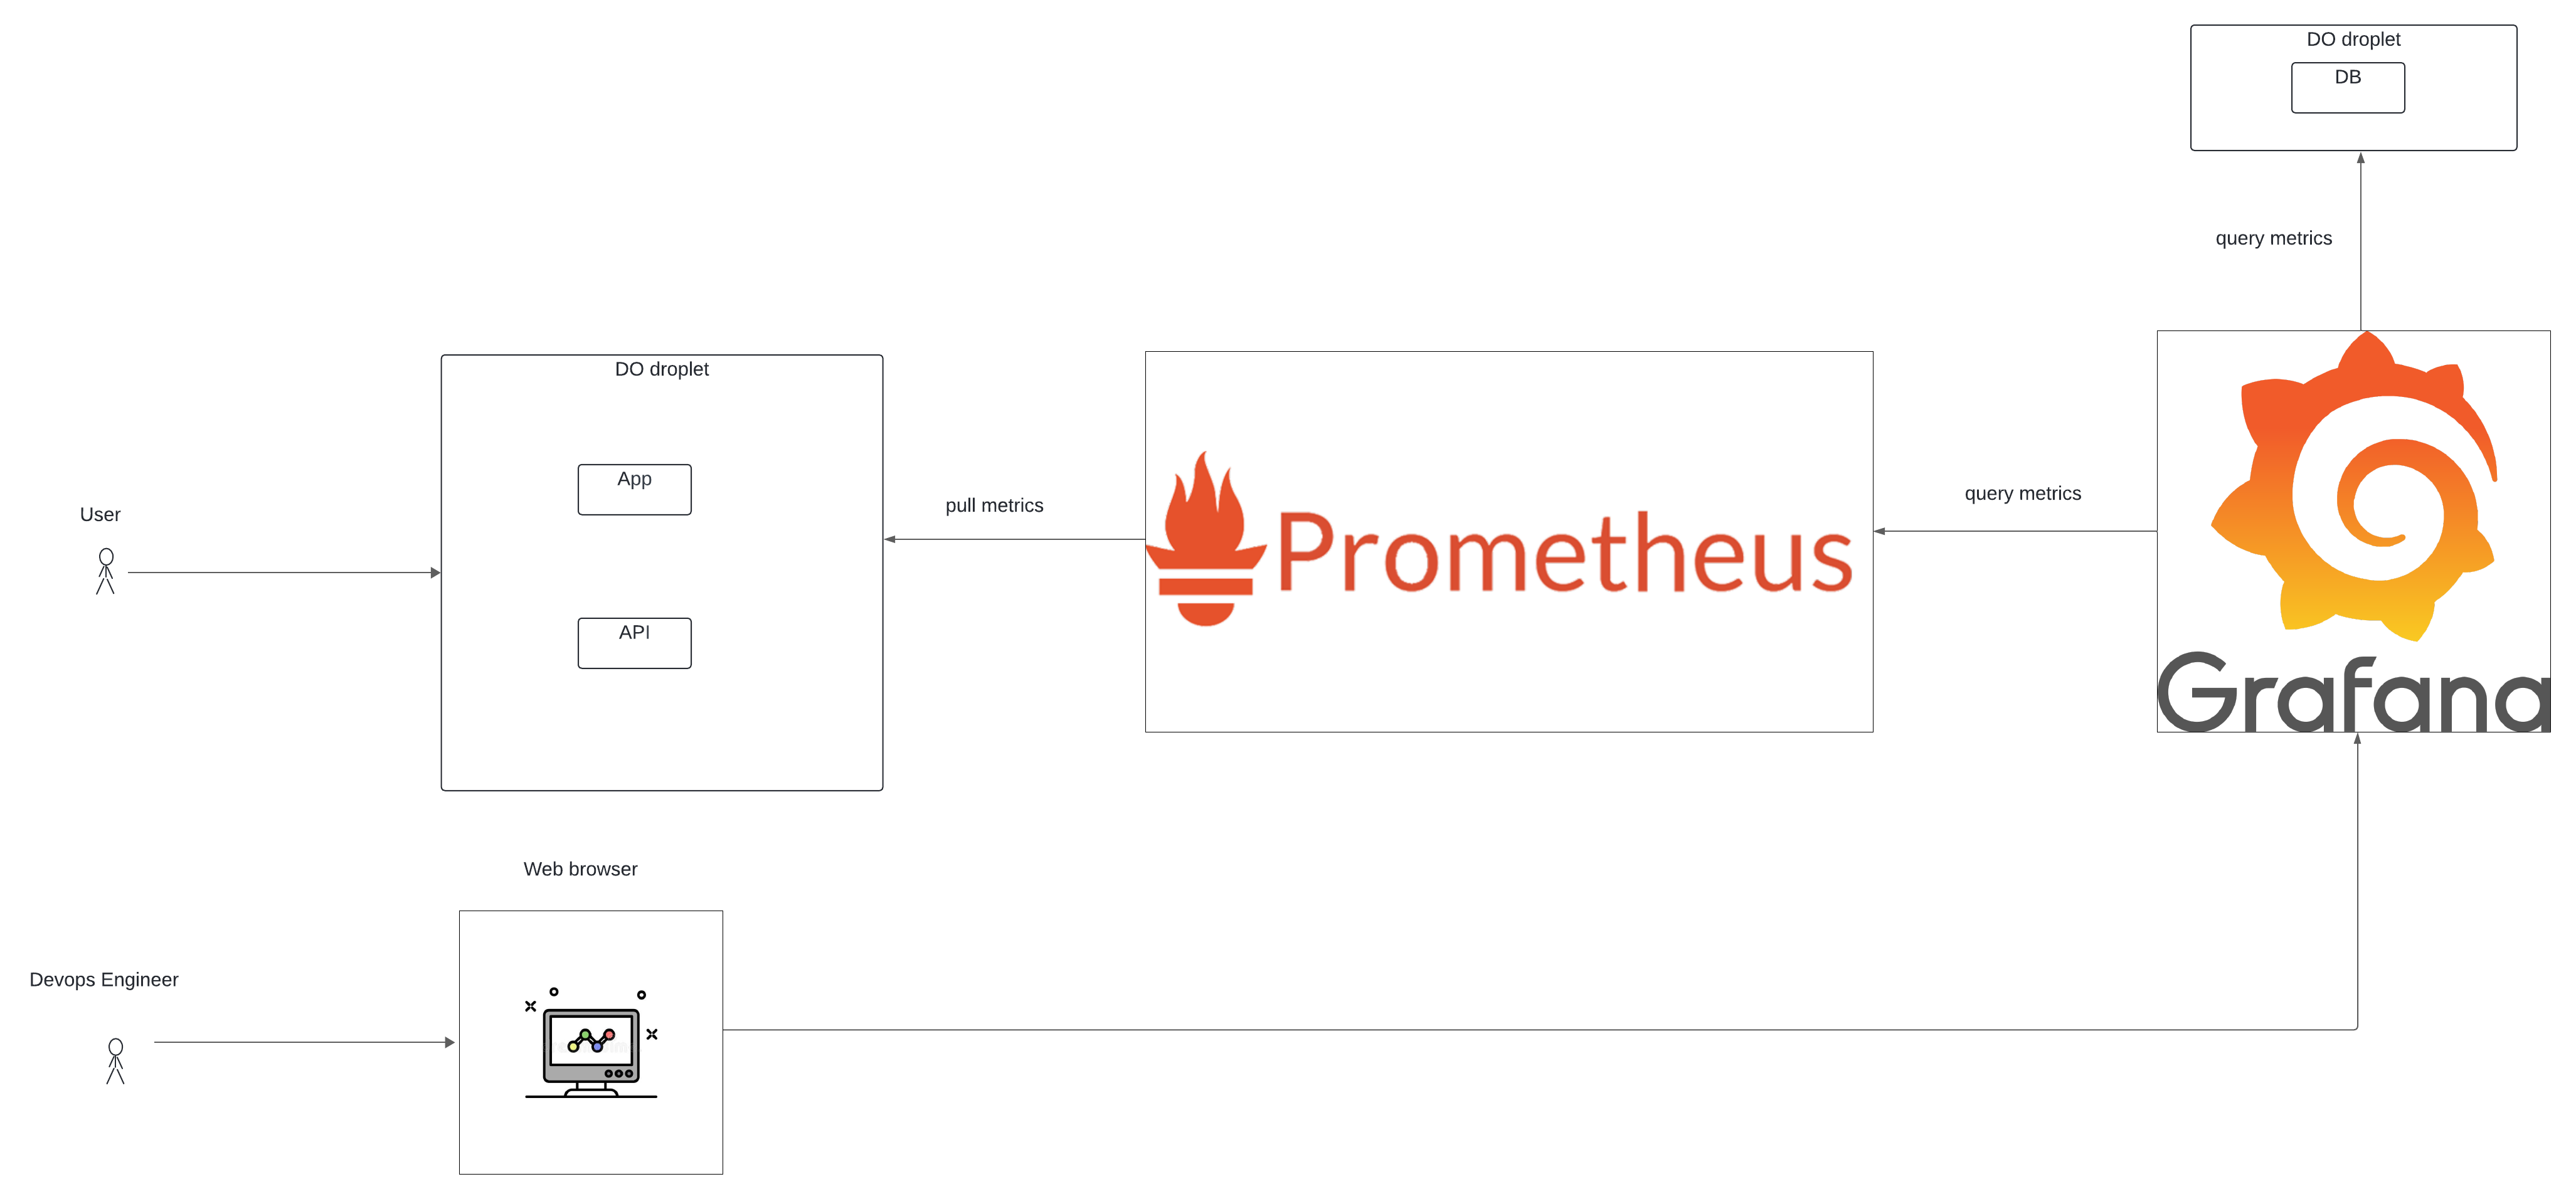
\includegraphics[scale = 0.3]{images/grafana.png}}
    \caption{Monitoring stack}
    \label{fig:monitoring-stack}
\end{figure}

\subsection{Logging}\label{sec:logging-architecture}

In Figure \ref{fig:elk-stack}, you can see how our ELKB stack is structured to ship logs to Elasticsearch and further analyze them.
\begin{figure}[H]
    \centering
    \hbox{\hspace{-6em}
    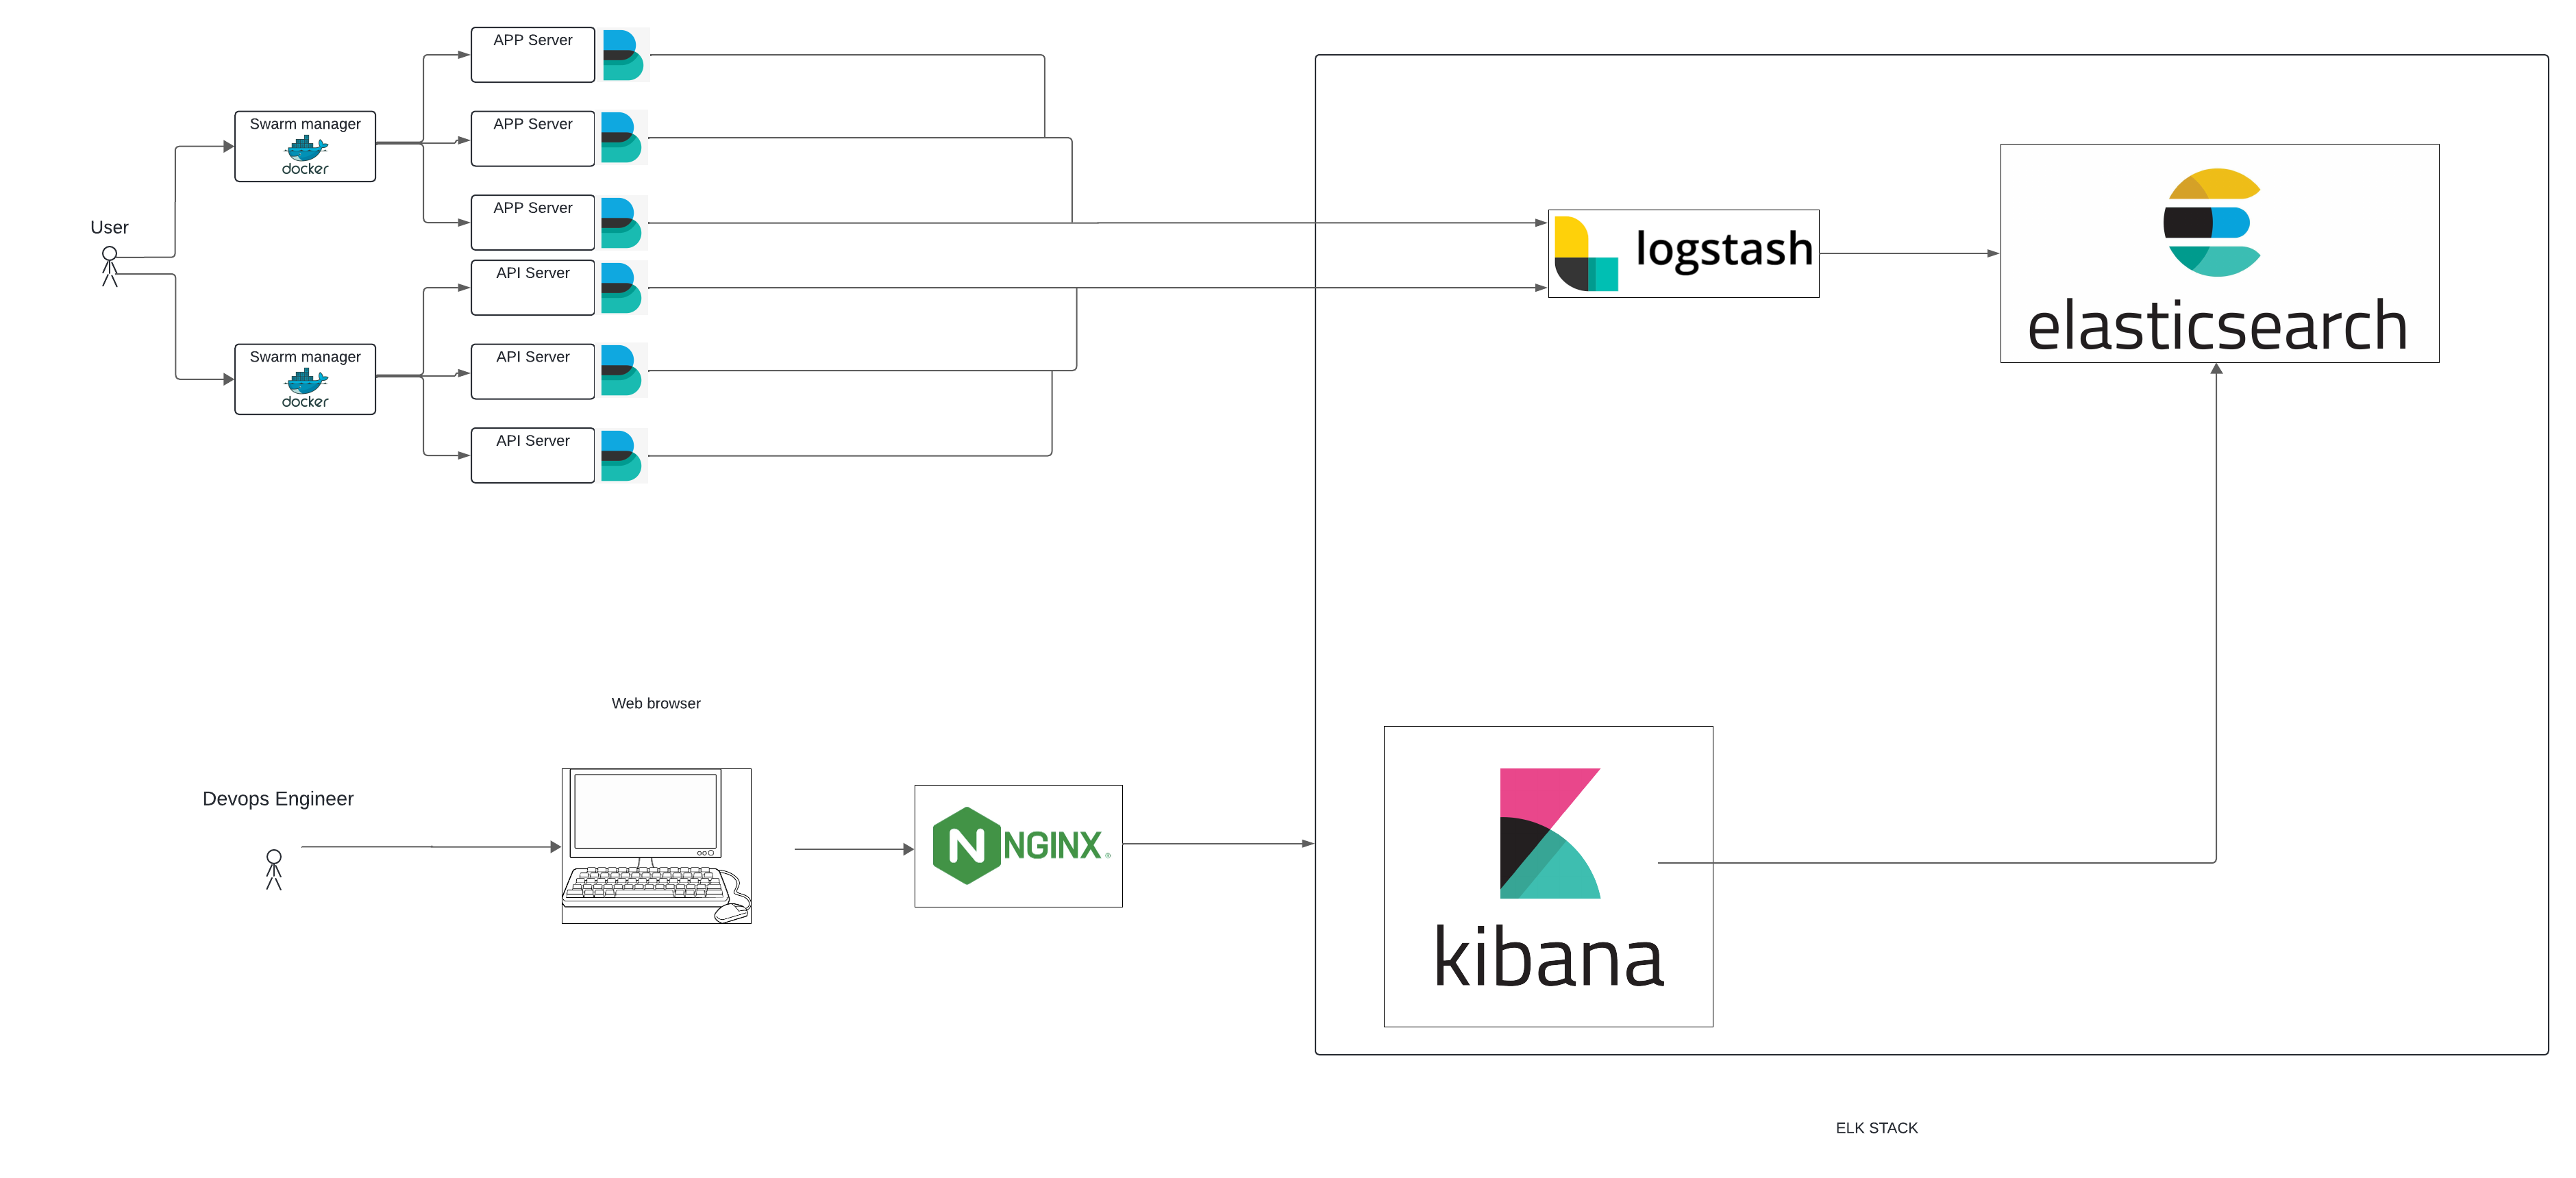
\includegraphics[scale = 0.37]{images/elk.png}}
    \caption{ELK stack}
    \label{fig:elk-stack}
\end{figure}

What enables the Filebeat to ship logs is a label tag added to our \textit{App} and \textit{API} services which enables Filebeat to autodiscover logs from those containers which has that option enabled. Filebeat will collect logs only containing a timestamp, which are those generated by the logger of our code, and ship them to Logstash where they will be further processed to be outputted to Elasticsearch. Finally, the Devops engineer can analyze and visualize these logs through Kibana through their browser, where the stack will be reversed proxied by Nginx for authentication reasons. \bigskip

\subsection{Development Dependencies}
We used Git and GitHub as the development version control and collaboration tools, and GitHub Organizations to manage the project with the "Projects" feature. 
GitHub Actions and Sonarcloud were used with workflows on pull requests to the \textit{main} branch, automating the CI/CD process and analysis of code quality.\bigskip

We used Terraform as the IaC, allowing for a simple IaC setup, with a \textit{tfvars} file to include environment variables efficiently.
All processes in the system are containerized with Docker to work without any dependency issues, using mainly docker-compose to orchestrate the services.\bigskip


\subsection{Runtime Dependencies}
The application is hosted in a Linux server inside a DigitalOcean droplet, where it is containerized with Docker.
The application and API connect to a Postgres database with GORM, a Golang ORM framework.
The database can easily be replaced due to a volume connected to the container storing the data.
The application and API are built with Golang and utilize the \textit{Gin} dependency, an HTTP web application package.


% Not really correct anymore, since the postgres is in an external server now:
% \begin{figure}[H]
%     \centering
%     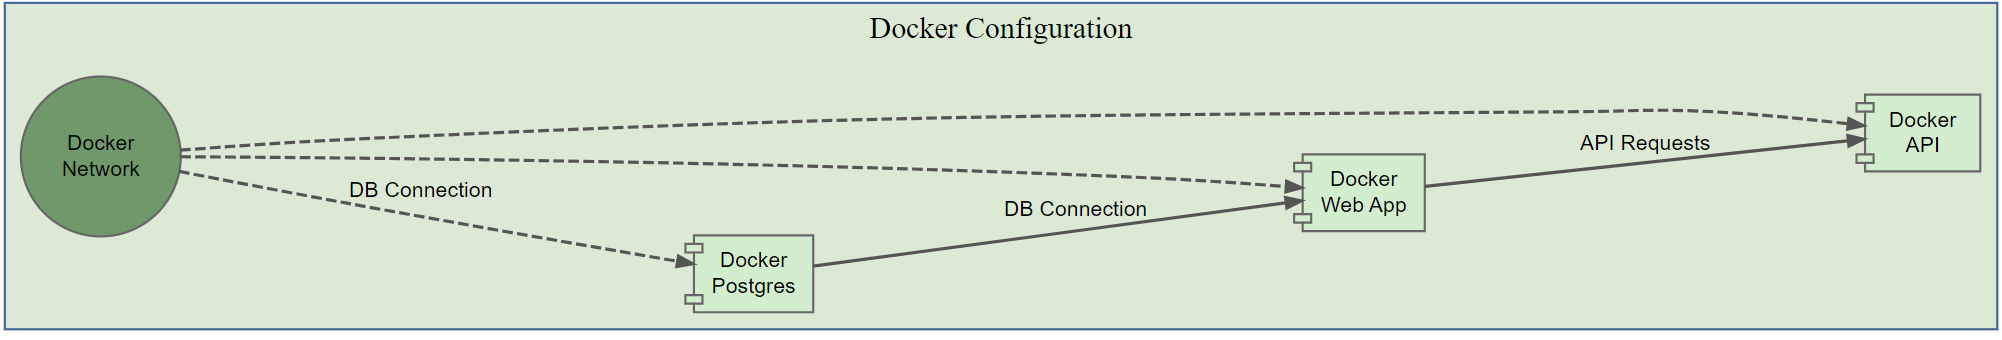
\includegraphics[width=\textwidth]{images/dockerconfig.png}
%     \caption{Docker Configuration}
% \end{figure}


\section{Important interactions of subsystems}

\subsubsection{Information Flow of the Web Application}
The diagram in Figure \ref{fig:seq-diagram-infoflow} showcases the system traversal of submitting a message.
When a user submits a message, the system makes a POST request to our web server, which routes the request to the controller, where it performs all the logic.
Afterwards, the proper status code is returned.
% link for the UML diagrams: \href{https://drive.google.com/file/d/1xU3Uf7EZC5fq4Bzw-O73jOwjMg971a8d/view?usp=sharing}{link1},\href{https://drive.google.com/file/d/1vgYJsYiDPGsxxs7oxMblu9runmONP_LT/view?usp=sharing}{link2}

\begin{figure}[H]
    \centering
    \fbox{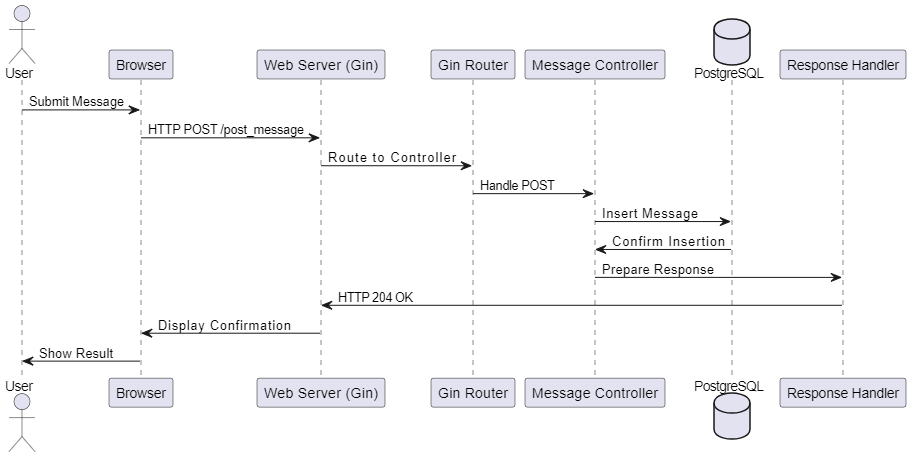
\includegraphics[width=\textwidth]{images/uml-seq-infoflow.png}}
    \caption{Sequence diagram of information flow of submitting a message in the application.}
    \label{fig:seq-diagram-infoflow}
\end{figure}

\subsubsection{Flow of API Endpoints}
Figure \ref{fig:seq-diagram-register} displays how the simulator traverses the register endpoint, including exception handling of unfilled register form and username already registered.

\begin{figure}[H]
    \centering
    \fbox{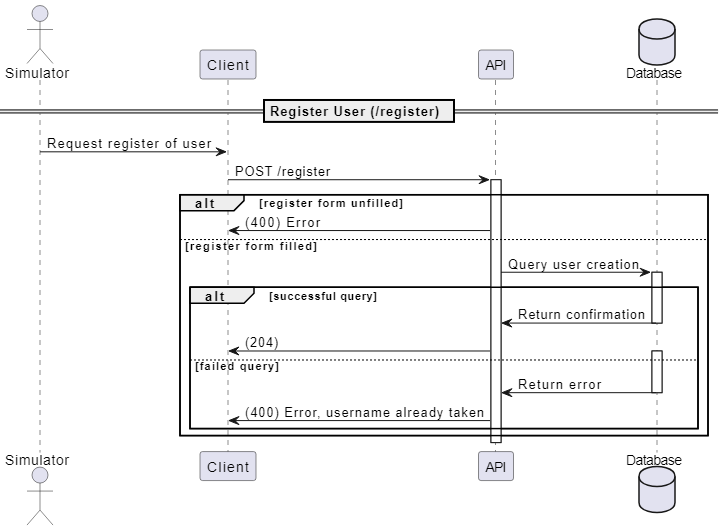
\includegraphics[width=0.7\textwidth]{images/uml-seq-register.png}}
    \caption{Sequence diagram displaying the traversal of the \texttt{POST /register} endpoint of the API.}
    \label{fig:seq-diagram-register}
\end{figure}

\begin{figure}[H]
    \centering
    \fbox{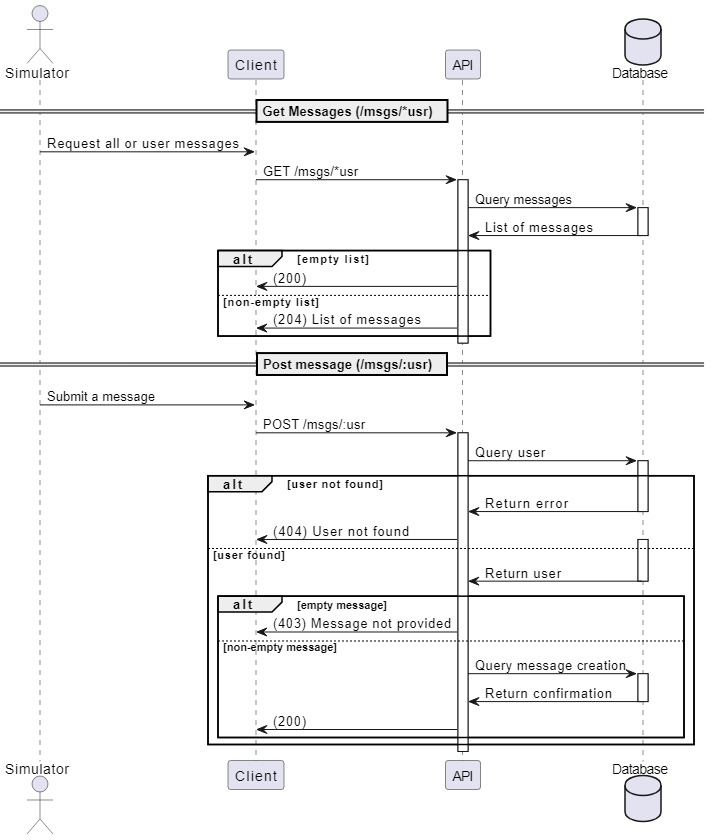
\includegraphics[width=0.75\textwidth]{images/uml-seq-message.png}}
    \caption{Sequence diagram displaying the traversal of the \texttt{/msgs} endpoints, including \texttt{GET /msgs/*usr} and \texttt{POST /msgs/:usr}, of the API.}
    \label{fig:seq-diagram-message}
\end{figure}

\newpage

Figure \ref{fig:seq-diagram-message} displays the traversal of the \texttt{/msgs} endpoints, including error handling with unregistered users and empty messages.
An important distinction is between the \texttt{usr}, where \texttt{*} indicates an optional user (fetching all messages if not provided), and \texttt{:} indicates a required user.

Figure \ref{fig:seq-diagram-follow} depicts the traversal of the \texttt{/fllws} endpoints, error handling at unregistered users, insufficient JSON format for the ORM, and if the query fails.
Unsuccessful follow will return 400, and unsuccessful unfollow will return 403.

\begin{figure}[H]
    \centering
    \fbox{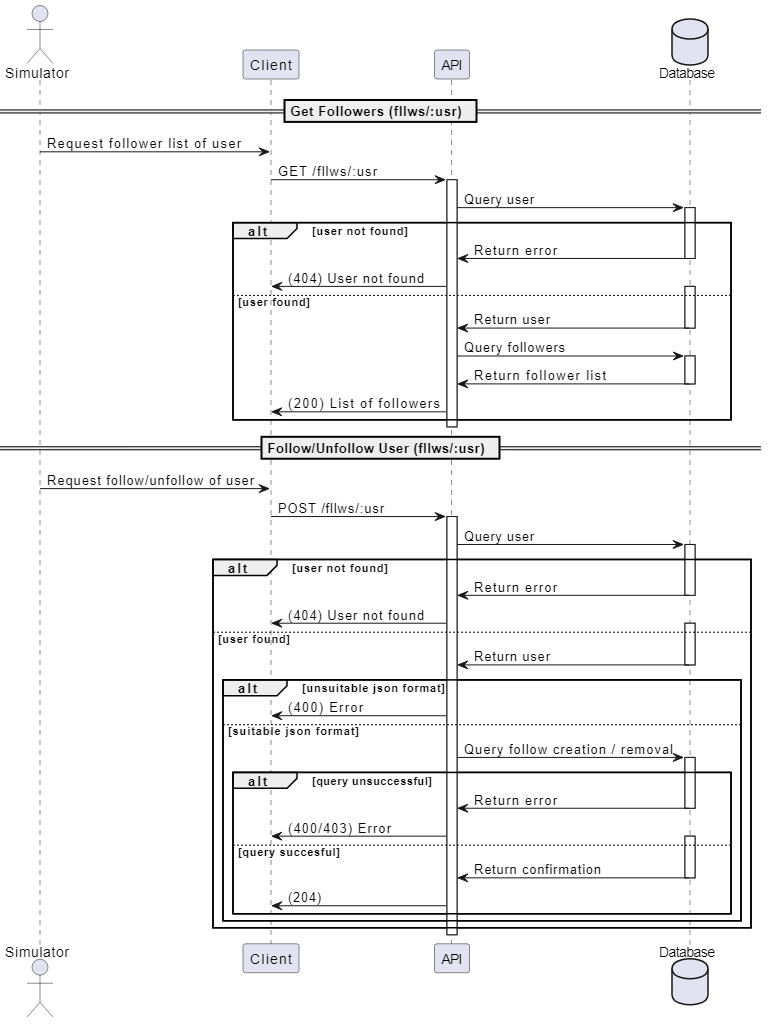
\includegraphics[width=0.8\textwidth]{images/uml-seq-follow.png}}
    \caption{Sequence diagram displaying the traversal of the \texttt{/fllws} endpoints, including \texttt{GET fllws/:usr} and \texttt{GET /fllws/:usr}, of the API.}
    \label{fig:seq-diagram-follow}
\end{figure}

\section{Current state of the system}
\hl{Include SonarCloud probably, how it currently looks and}


Ideas:
\begin{itemize}
    
\item Static Analysis:
\item Present results from static analysis tools to discuss code quality, potential bugs, and security issues.
\item Mention any significant findings and how they impact the overall system.
\item Quality Assessment:
\item Discuss methods used for assessing the quality of the application (e.g., code reviews, testing coverage).
\item Summarize the current quality metrics and any goals or benchmarks your team is aiming to achieve.
\item Using Prometheus, document current performance metrics of the system, analyzing aspects such as response times, system throughput, and error rates.

\end{itemize}

\begin{itemize}

    \item[1.] Static Analysis Results:
Static analysis tools examine your code without executing it to find potential issues. Here's what to look at:

\item Code Quality Metrics:
\item Complexity: Measures how complex the logic in your codebase is. Lower complexity often correlates with easier maintenance.
\item Code Style Compliance: Checks adherence to coding standards and conventions, which help in maintaining code consistency.
\item Potential Bugs: Identification of code patterns that could lead to errors.
\item Code Smells: Highlight suboptimal code practices that might not cause bugs but could reduce code quality or increase complexity.
\item Security Vulnerabilities:
\item Known Vulnerabilities: List of known vulnerabilities in your dependencies or your code that could be exploited.
\item Security Hotspots: Areas in the code that require a manual review to ensure they are secure.
\item[2.] Quality Assessments:
Quality assessments go beyond static code analysis by incorporating other factors such as unit test coverage and integration test results.


\item Test Coverage:
\item Unit Test Coverage: Percentage of your codebase covered by unit tests. High coverage can reduce the likelihood of bugs making it to production.
\item Integration Test Results: These tests cover interactions between modules or services and help identify issues in the way components integrate.
\item Performance Metrics:
\item Response Times: Average time it takes for your system to respond to user actions.
Resource Usage: Usage statistics for CPU, memory, and other resources. High usage might indicate a need for optimization.
\item Dependency Health:
\item Outdated Libraries: Using outdated libraries can expose your system to security vulnerabilities and compatibility issues.
License Compliance: Ensuring that all library licenses comply with your project's licensing.
\item 3. System Observability and Monitoring:
Logs Analysis: Insights into errors and unusual system behavior captured in logs.
Metrics Dashboard: A real-time dashboard showing key performance metrics.
Alerts History: Review of past alerts to understand recurring issues or spikes in resource usage.
\item 4. Development Practices:
Code Review Practices: Regular code reviews help maintain code quality and mentor junior developers.
Build and Deployment Frequency: Frequency of deployments can indicate the agility and health of the development process.
Feature Development Speed: How quickly new features move from conception to production
% A description and illustration of the:
% - Design and architecture of your ITU-MiniTwit systems
% - All dependencies of your ITU-MiniTwit systems on all levels of abstraction and development stages. That is, list and briefly describe all technologies and tools you applied and depend on.
% - Important interactions of subsystems
%    - For example, via an illustrative UML Sequence diagram that shows the flow of information through your system from user request in the browser, over all subsystems, hitting the database, and a response that is returned to the user.
%    1- Similarly, another illustrative sequence diagram that shows how requests from the simulator traverse your system.
% - Describe the current state of your systems, for example using results of static analysis and quality assessments.
\end{itemize}


\chapter{Process' perspective}
% This perspective should clarify how code or other artifacts come from idea into the running system and everything that happens on the way.
% In particular, the following descriptions should be included:
% - A complete description of stages and tools included in the CI/CD chains, including deployment and release of your systems.
% - How do you monitor your systems and what precisely do you monitor?
% - What do you log in your systems and how do you aggregate logs?
% - Brief results of the security assessment and brief description of how did you harden the security of your system based on the analysis
% - Applied strategy for scaling and upgrades
% In case you have used AI-assistants during your project briefly explain which system(s) you used during the project and reflect how it supported/hindered your process.

\section{CI/CD Chain}
We implemented a GitHub Actions workflow to automate the process of testing, building and deploying the most recent version of Minitwit, set to execute on each pull request to the \textit{main} branch of our GitHub repository.
The workflow is separated into three jobs: \textit{BuildAndTest}, \textit{Deploy}, and \textit{Release}, which are executed sequentially, each dependent on the last executing successfully. \bigskip

A comprehensive deployment diagram describing the build and deployment part of the CI/CD applied with GitHub Actions is displayed in Figure \ref{fig:deployment-cicd-minimal}.\bigskip

\begin{figure}
    \centering
    \includegraphics[width=\linewidth]{images/uml-deployment-githubactions.png}
    \caption{Deployment Diagram of deploying with a pull request or manually on GitHub Actions.}
    \label{fig:deployment-cicd-minimal}
\end{figure}

\newpage

\subsection{Jobs}
\subsubsection{BuildAndTest}
All relevant images are built and pushed to the Docker hub and then run and tested to ensure the system is working. The key steps are as follows:

\begin{enumerate}
    \item \textbf{Checkout} 
    \begin{itemize}
        \item Uses \texttt{actions/checkout@v2} to fetch the codebase from the repository.
    \end{itemize}
    
    \item \textbf{Environment Setup} 
    \begin{itemize}
        \item Dynamically creates a \texttt{.env} file with database configurations sourced from GitHub secrets.
    \end{itemize}
    
    \item \textbf{Docker Operations}
    \begin{itemize}
        \item Logs into Docker Hub using credentials from GitHub secrets to push built images, including:
        \begin{itemize}
            \item The application image
            \item API image
            \item A test database image
        \end{itemize}
    \end{itemize}
    
    \item \textbf{Python Setup and Dependency Installation}
    \begin{itemize}
        \item Configures the Python environment and installs necessary dependencies to ensure consistent testing conditions.
    \end{itemize}
    
    \item \textbf{Testing}
    \begin{itemize}
        \item Executes integration tests by setting up the application and its dependencies in Docker containers.
        \item Conducts API tests and application-specific tests to ensure functionality and reliability.
    \end{itemize}
\end{enumerate}

\subsubsection{Deploy}
The \textbf{Deploy} job is activated on successfully completing the \textbf{BuildAndTest} job.
It manages the deployment of the application to the remote server where the application is hosted.
The steps conducted are the following:

\begin{enumerate}
    \item \textbf{Checkout} 
    \begin{itemize}
        \item Retrieves the latest codebase from the repository, uses \texttt{actions/checkout@v2} similar to the first job.
    \end{itemize}
    \item \textbf{SSH Configuration} 
    \begin{itemize}
        \item Prepares SSH keys to establish a secure connection to the deployment server.
    \end{itemize}
    
    \item \textbf{Deployment Execution}
    \begin{itemize}
        \item Updates environmental configurations and transfers necessary files to the server using SCP.
        \item Pull the latest Docker images from the Docker Compose file.
        \item Deploys the images using Docker Stack, effectively updating the running application on all servers in the Docker swarm.
    \end{itemize}
\end{enumerate}

 \subsubsection{Release}
 After the previous jobs have been successfully completed, this job manages software versioning and public release.

 \begin{enumerate}
    \item \textbf{Version Calculation:}
    \begin{itemize}
        \item Executes a script to determine the new version number for automated version tracking.
    \end{itemize}
    
    \item \textbf{GitHub Release Creation:}
    \begin{itemize}
        \item Uses \texttt{actions/create-release@v1} to create a formal release on GitHub.
        \item Tags the release with the new version number and provides release notes outlining the changes in this version.
    \end{itemize}
\end{enumerate}

\section{Monitoring}
For monitoring, we use Prometheus to collect metrics and integrate them with Grafana to visualize key metrics live. Additionally, Grafana queries the database to visualize the data stored.
We have two dashboards, one monitoring the API and the other the database.
DigitalOcean also includes infrastructure monitoring with real-time bandwidth, CPU usage, and disk I/O graphs, as depicted in Figure \ref{fig:do-monitoring}.

\begin{figure}[H]
    \centering
    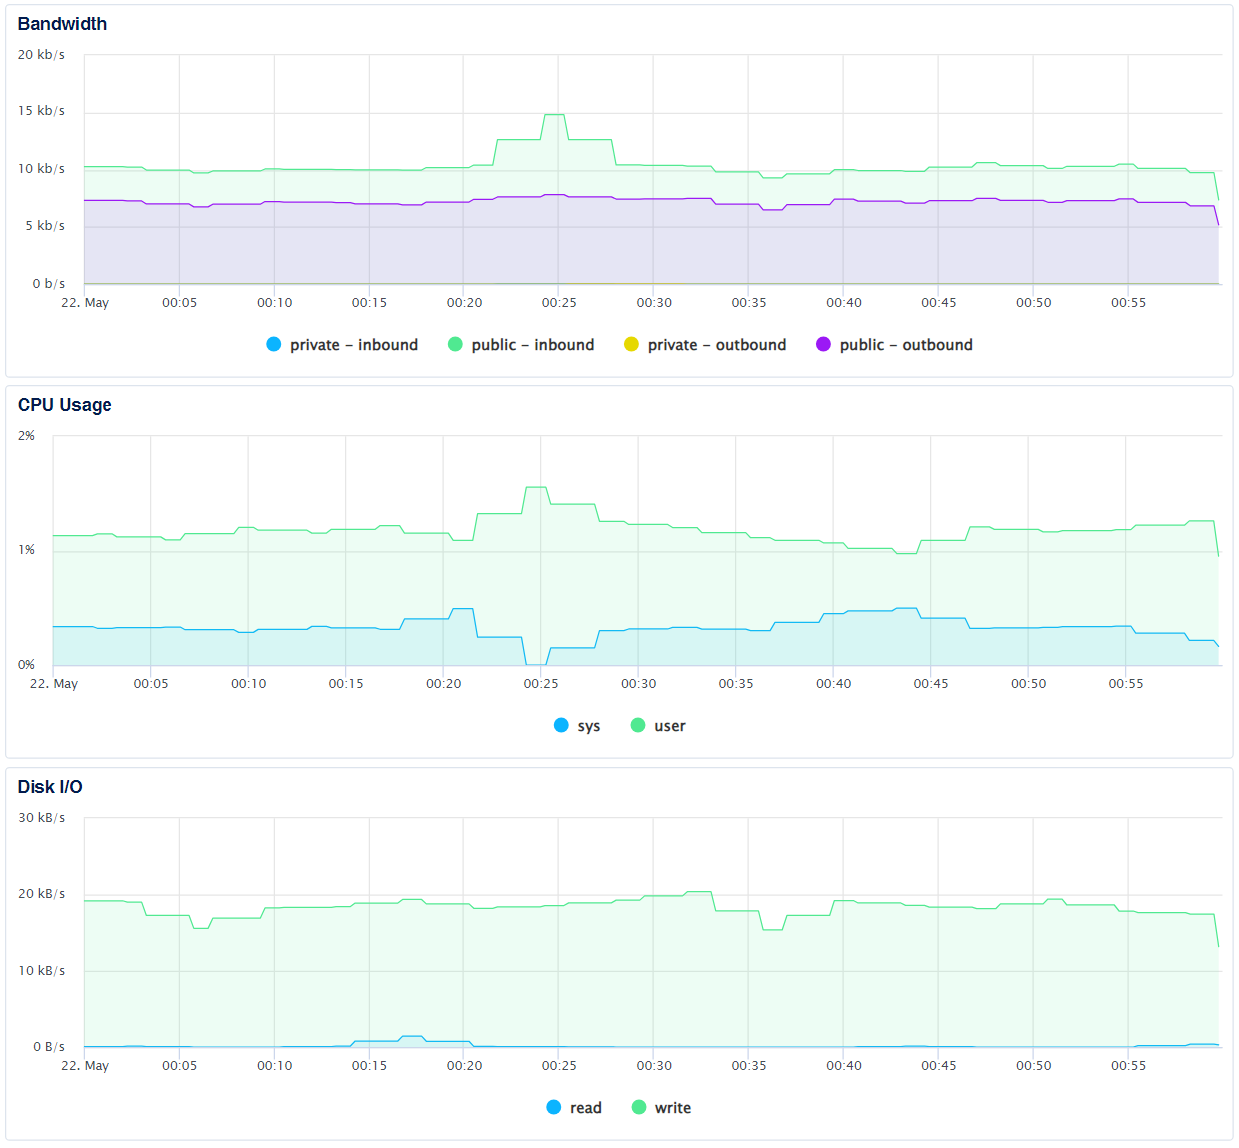
\includegraphics[width=0.7\linewidth]{images/do-monitoring.png}
    \caption{DigitalOcean Monitoring}
    \label{fig:do-monitoring}
\end{figure}

\subsection{API dashboard}
The API dashboard mainly focuses on determining which HTTP requests are incoming from the API, prioritized due to the simulator using the API.
% Comment from here if necessary -------------------------------------------------------
The dashboard collects data from Prometheus.
The monitoring uses an application monitoring strategy, monitoring how well the API responds to requests and which requests occur.
It also includes passive monitoring by sniffing the simulated users' HTTP requests and is considered proactive monitoring since it measures application performance.
The metrics from Prometheus are pulled from the code, which pushes all metrics into an API endpoint, so it is somewhat of a hybrid monitoring, although mostly pull-based and whitebox.
% Uncomment from here if necessary -----------------------------------------------------
% Below is a description of the dashboard:
% \begin{itemize}
%     \item \textbf{Data source:} Prometheus
%     \item \textbf{Monitoring strategy:} application monitoring
%     \item \textbf{Passive or Active:} Passive
%     \item \textbf{Stage in maturing model:} Proactive
%     \item \textbf{Push or pull-based:} Hybrid, mainly pull-based
%     \item \textbf{Whitebox or blackbox:} whitebox
% \end{itemize}
Figure \ref{fig:api-dashboard} displays the API monitoring dashboard.

\begin{figure}[H]
    \centering
    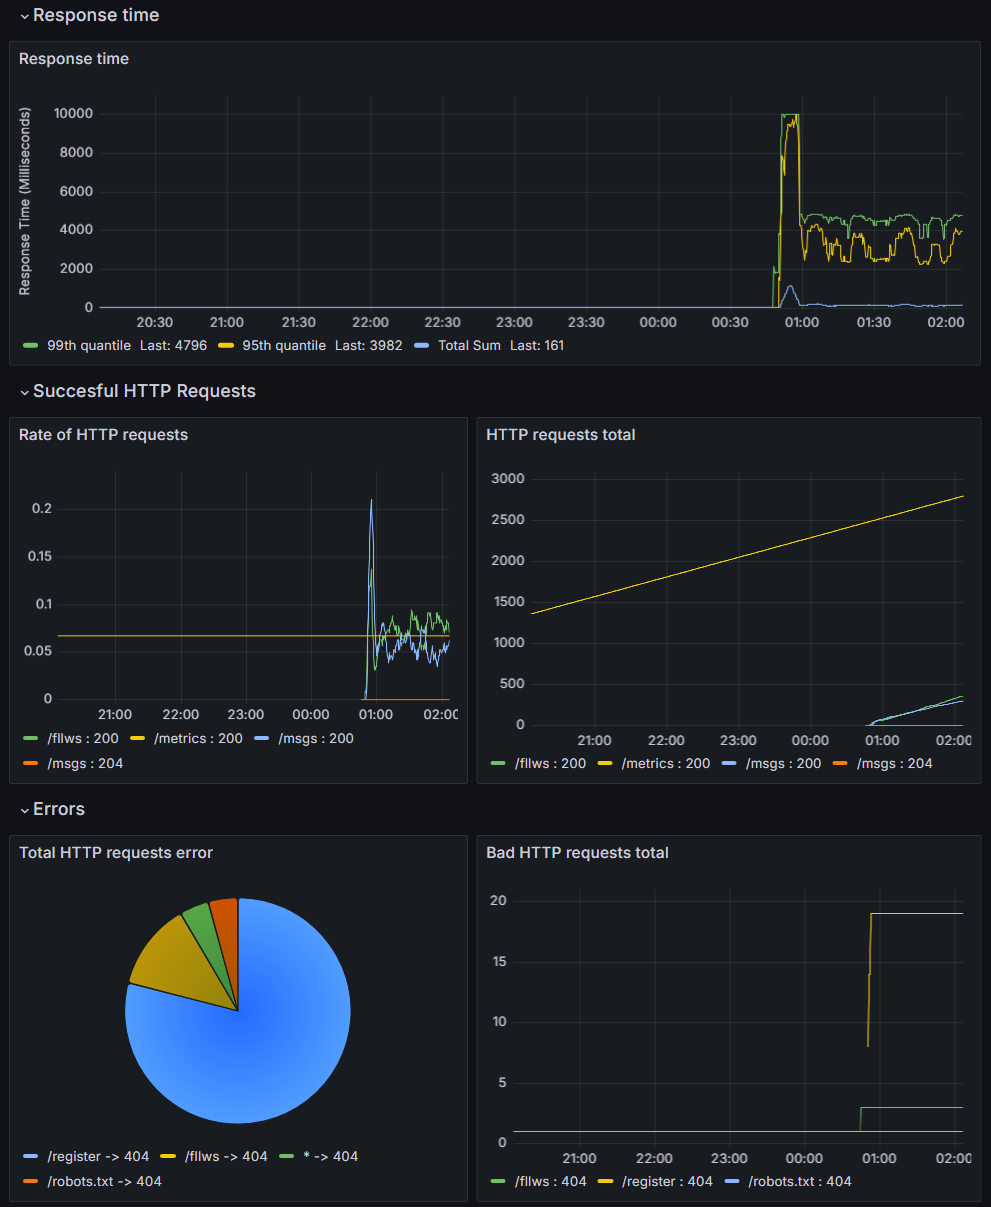
\includegraphics[width=0.7\linewidth]{images/api-dashboard.png}
    \caption{API Dashboard in Grafana}
    \label{fig:api-dashboard}
\end{figure}


%The following describes the different stats visualized in Grafana on the API dashboard:

% \begin{itemize}
%     \item \textbf{Response time:}
%     This chart displays the response times of requests over the past six hours, with separate lines for the slowest 95th and 99th percentile requests.

%     \item \textbf{Rate of HTTP requests:}
%     Shows the number of HTTP requests per second, categorized by endpoints.
    
%     \item \textbf{HTTP Requests Total:}
%     Shows the total number of HTTP requests received, categorized by endpoints.
    
%     \item \textbf{Total HTTP request errors:}
%     Shows a chart of total HTTP request errors by endpoint.
    
%     \item \textbf{Bad HTTP request total:}
%     Shows the total number of bad requests made, by endpoint.
% \end{itemize}

\subsection{Database dashboard}
The database dashboard visualizes stats about what is currently obtained in the database.
% Comment from here if necessary -------------------------------------------------------
This is done by querying the database directly from Grafana.
The database monitoring acts like a 'monitoring the business' strategy by visualizing information about the number of users and messages there are and revealing distributions that may be useful for business.
The dashboard includes passive monitoring by sniffing information about the users registered to the system.
It is also considered proactive monitoring, measuring application performance.
The database statistics are considered pull-based since the database is queried to and, therefore, pulled from, and it is considered whitebox.
% Uncomment from here if necessary -----------------------------------------------------
% Below is a description of the dashboard:
% \begin{itemize}
%     \item \textbf{Data source:} Postgres
%     \item \textbf{Monitoring strategy:} monitoring the business
%     \item \textbf{Passive or active:} passive
%     \item \textbf{Stage in maturing model:} proactive
%     \item \textbf{Push or pull-based:} pull-based
%     \item \textbf{Whitebox or blackbox:} whitebox
% \end{itemize}
Figure \ref{fig:db-dashboard} displays the database monitoring dashboard.

\begin{figure}[H]
    \centering
    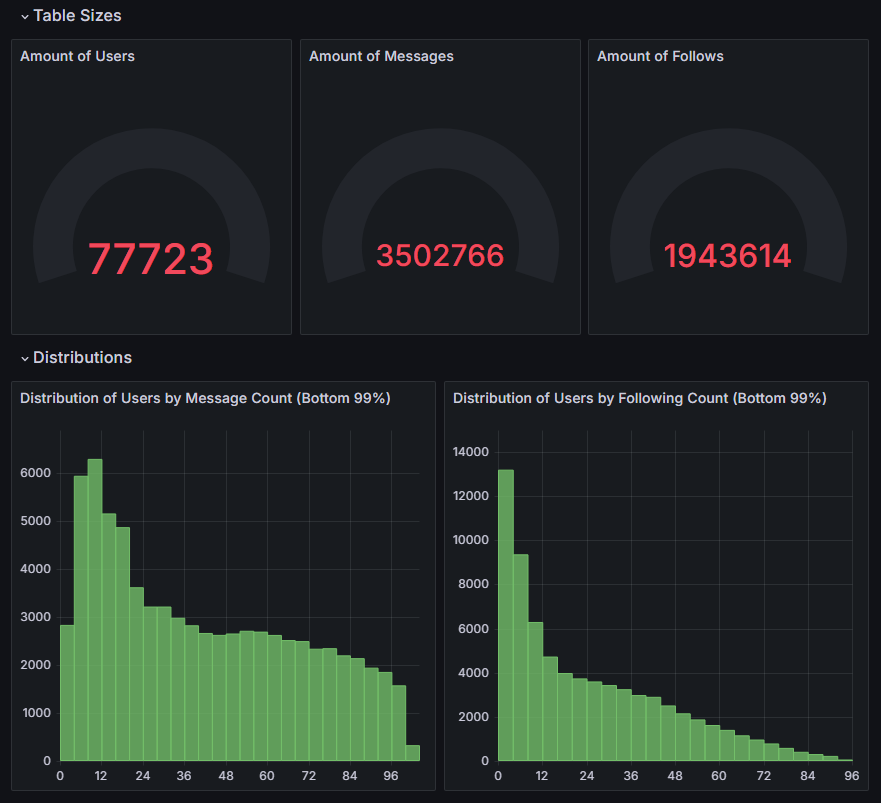
\includegraphics[width=0.8\linewidth]{images/database-dashboard.png}
    \caption{Database Dashboard in Grafana}
    \label{fig:db-dashboard}
\end{figure}

% The following describes the different stats visualized in Grafana on the database dashboard:

% \begin{itemize}
%     \item \textbf{Amount of users:}
%     Gauge charting user count.
%     \item \textbf{Amount of messages:}
%     Gauge charting message count.    
%     \item \textbf{Amount of follows:}
%     Gauge charting count of follows between users.
%     \item \textbf{Distribution of users by message count:}
%     Bar chart showing count of users by number of messages.
%     \item \textbf{Distribution of users by following count:}
%     Bar chart showing count of users by how many they follow.
% \end{itemize}



\section{Logging}

We log the main events of our application and API; we mainly use 4 levels for this purpose: info, debug, error, and fatal. We used the “info” level to communicate the events in a general level of how things are happening; “debug” for debugging purposes, how parameters are being changed and passed; “error” when the program encounters some non-fatal errors for example, in our Go app when the “err” parameter is not nil we notify it with the error level; finally “fatal” is used for errors that halt or crashes the application. \bigskip

All logs are collected in a single index pattern from all sources from the “app” and “application.
We can distinguish the sources in Kibana because you can see from which folder and which file the log is generated, depicted in Figure \ref{fig:kabana-logs}.
\begin{figure}[H]
    \centering
    \hbox{\hspace{-5em}
    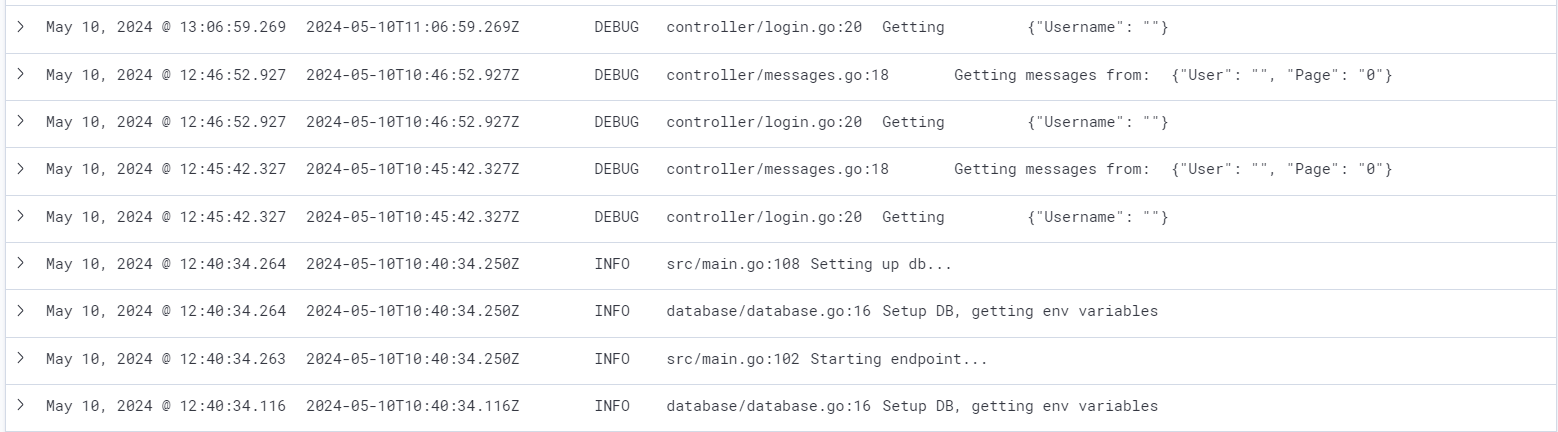
\includegraphics[scale = 0.6]{images/kibana.png}}
    \caption{Logs from Kibana}
    \label{fig:kabana-logs}
\end{figure}

\section{Security assessment}
The application components are as described in chapter~\ref{chap:System's Perspective} section 
~\ref{sec:Design and architecture of the Minitwit system}. 

The user data that we store in our database are username, password, and email.
The username and email are public information and are therefore not sensitive data.
Depending on the user, and if they are reusing their password on multiple applications, the password is not sensitive data.

\begin{figure}[H]
    \centering
    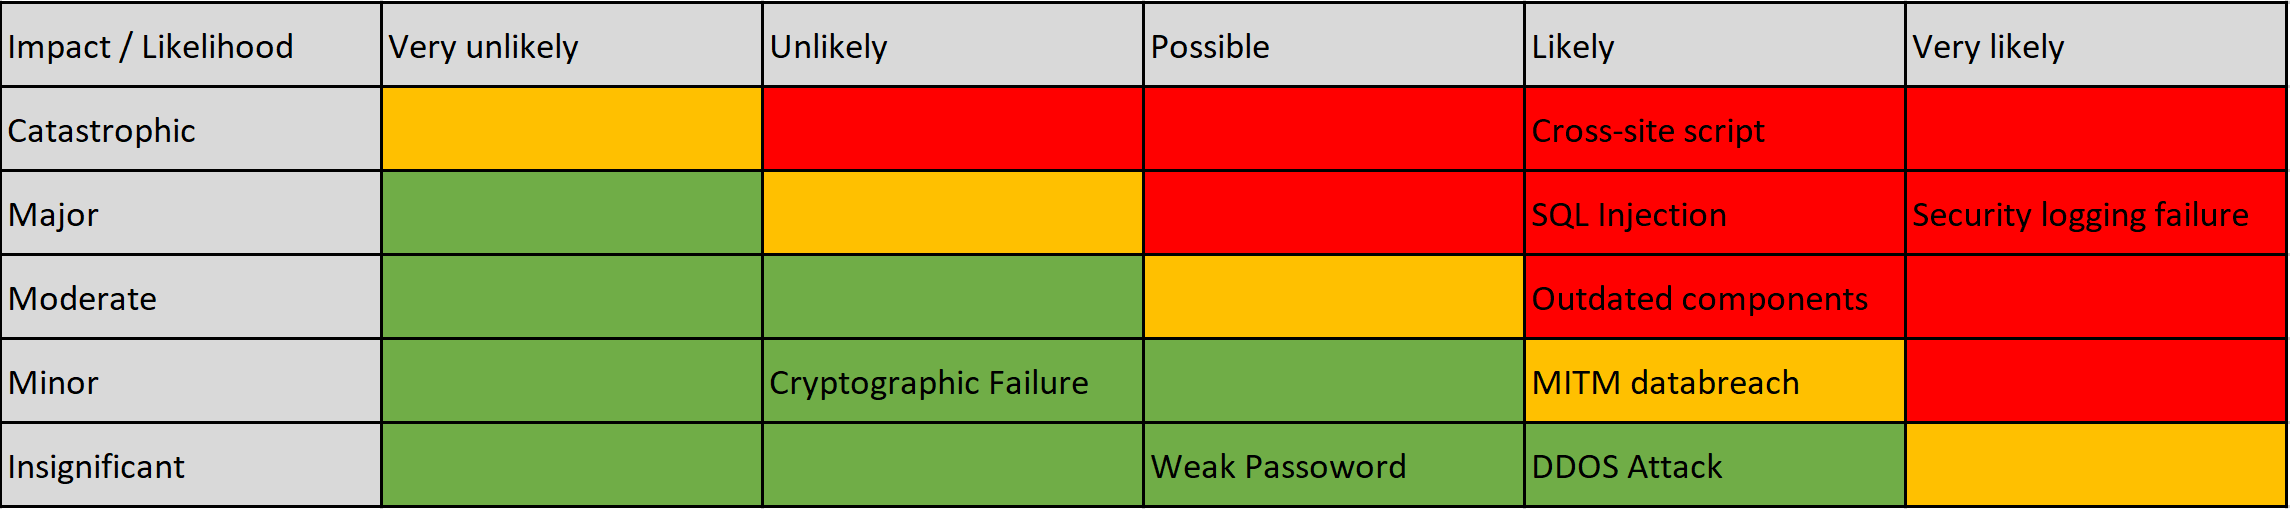
\includegraphics[width=1.0\textwidth]{images/SecRiskAssMatrix.PNG}
    \caption{Security risk assessment matrix\cite{owasp2024}\cite{comparitech2024}}
    \label{fig:security matrix}
\end{figure}


\section{Scaling strategy}
The system induced both horizontal and vertical scaling.
Horizontal scaling is provided by utilizing Docker Swarm, with two additional worker replicas to assist the single web server in its tasks from the app and API, which can easily be scaled by increasing workers.
The web server is the manager who delegates tasks to the workers and also handles the tasks itself if delegation is unnecessary.
Furthermore, Docker Swarm also functions as a backup system; if a node in the system crashes, the others will help it recreate.\\
\\
Vertical scaling was utilized when adding the ELK stack.
Elasticsearch was very performance-heavy; as a quick solution, the web server was scaled vertically with more memory from 1 GB to 8 GB and more processing power from 1 virtual CPU to 4 virtual CPUs.
This solution was very simple but cannot be as easily expanded and is not as preferred.

\chapter{Lessons Learned Perspective}

\section{Evolution and refactoring}
We learned the whole process of making software evolve to adapt to the best technologies. We refactored a legacy Python application to Go.\bigskip

The major issue we found is how to map the functionalities written in Python against how it would be written in Go, since they are very different. What we learned is that when you have to migrate a codebase from a language to another, the best thing to do is to go with small steps, first, map the core functionalities, test it and develop the rest of functionalities incrementally to ensure correct integrations.
\section{Operation}
Creating the workflow for our pipelines was easy, it was just a 4 step process: build, test, deploy and release operations.
The main issues we found while trying to implement it were in test and releasing. \bigskip

For the testing part, it was difficult since we wanted to keep the test provided by the course which were in Python, we could have written some test in Go and run some Go command which would run them automatically, but since we decided to keep the Python test, we had to have running instances of images for the APP and API tests. But the main problem we faced was that, once we had a running instances, these would be connecting to an already populated database image because the docker-compose file was connected to it, to fix this issue, we made 2 Docker Compose files, one for development and another for production, the development would have a database image, and when we bring up the instances for testing, we build the development file, and they will be connected to an empty database. \bigskip

For releasing, we didn't know how to update the release number after each deployment, we thought about using the tag of the commit for releases. Since we didn't find a way to get the tag number, we wrote a shell script where it would get the latest release of our application and update it for our newest release.
\section{Maintenance}
Keeping track of the logs can help us detect any bugs in the code and trace them so they can be fixed, assisting in maintenance.
Additionally, monitoring could check the performance of our endpoints and determine if any errors or unusual activity have occurred so we can take action if necessary.\bigskip
When scaling the application with Docker Swarm, we faced an issue where the Grafana dashboards and login credentials were removed due to creating a new container, which we fixed by adding a volume to the Grafana container.
Furthermore, Elasticsearch was very performance-heavy when adding the logging, so we upgraded the webserver host with more memory and CPU power.




% Describe the biggest issues, how you solved them, and which are major lessons learned with regards to:
% - evolution and refactoring
% - operation, and
% - maintenance
% of your ITU-MiniTwit systems. Link back to respective commit messages, issues, tickets, etc. to illustrate these.
% Also reflect and describe what was the "DevOps" style of your work. For example, what did you do differently to previous development projects and how did it work?

\chapter{Appendix}
\section{Sources}

\begingroup
\renewcommand{\bibname}{}
\printbibliography[heading=none]
\endgroup

% \begin{figure}
%     \centering
%     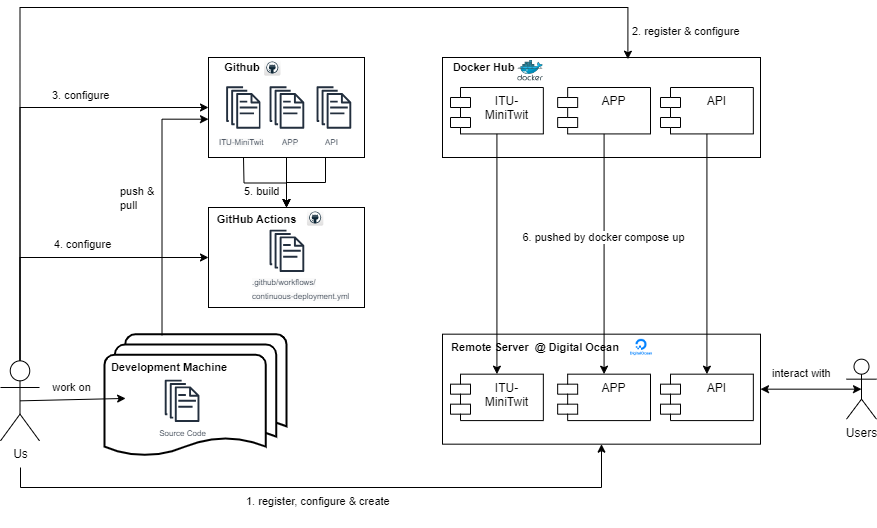
\includegraphics[width = \textwidth]{images/image5.drawio.png}
%     \caption{\href{https://drive.google.com/file/d/1UgSQr3RA1gUwPlpxuSjn5uB8MuakvssY/view?usp=sharing}{link}}
%     \label{fig:allocation-diagram-1}
% \end{figure}

% \begin{figure}
%     \centering
%     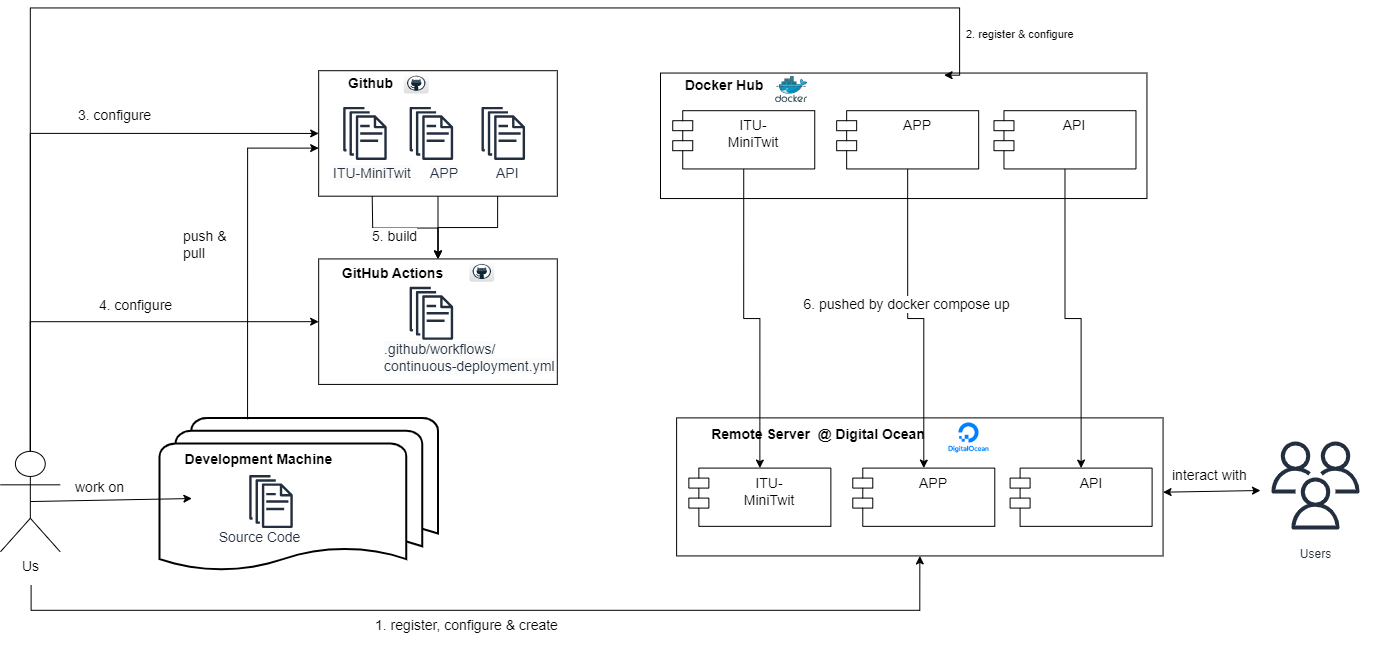
\includegraphics[width = 1.1\textwidth]{images/img5.drawio.png}
%     \caption{Allocation Diagram: \href{https://drive.google.com/file/d/1UgSQr3RA1gUwPlpxuSjn5uB8MuakvssY/view?usp=sharing}{link}}
%     \label{fig:allocation-diagram-2}
% \end{figure}

% \begin{figure}
%     \centering
%     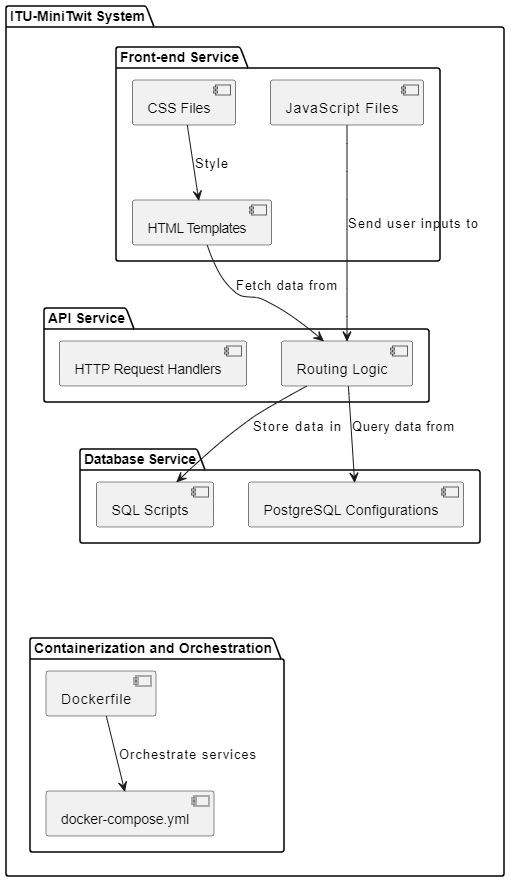
\includegraphics[width = 0.6\textwidth]{images/module.png}
%     \caption{Module Viewpoint of the MiniTwit System: \href{https://drive.google.com/file/d/1QDKjREb_C-90b0LAtigcrdJvNRZfml1a/view?usp=sharing}{link}}
%     \label{fig:module-viewpoint}
% \end{figure}

% This diagram illustrates the modular architecture of the MiniTwit system, highlighting the key components and their relationships. The system comprises the Front-end Service, API Service, Database Service, and Containerization and Orchestration. The Front-end Service provides the user interface, interacting with the API Service for data exchange. The API Service handles client-server interactions and communicates with the Database Service, which uses PostgreSQL for data storage. Containerization and orchestration are managed using Docker and Docker Compose to ensure isolated and efficient deployment of all services.

\end{document}
